%% ----------------------------------------------------------------
%% M A I N - F I L E 
%% ---------------------------------------------------------------- 

% Set up the document
\documentclass[a4paper, 11pt, oneside]{main} 
\graphicspath{{Figures/}} 
\usepackage[german]{babel} % ALLES SCHÖN DEUTSCH!

% Include any extra LaTeX packages required
\usepackage[square, numbers, comma, sort&compress]{natbib}  % Use the "Natbib" style for the references in the Bibliography

\usepackage{verbatim}  % Needed for the "comment" environment to make LaTeX comments

\usepackage{url}
\usepackage{natbib}

% Floating images and tables
\usepackage{float}

% to comment out entire sections
\usepackage{comment}

% to use listings
\usepackage{listings}

% Um Code hervorzuheben und umzufärben --------------
\usepackage{listings,xcolor}
\usepackage{inconsolata}

\definecolor{dkgreen}{rgb}{0,.6,0}
\definecolor{dkblue}{rgb}{0,0,.6}
\definecolor{dkyellow}{cmyk}{0,0,.8,.3}

\lstset{
  language        = php,
  basicstyle      = \small\ttfamily,
  keywordstyle    = \color{dkblue},
  stringstyle     = \color{red},
  identifierstyle = \color{dkgreen},
  commentstyle    = \color{gray},
  emph            =[1]{php},
  emphstyle       =[1]\color{black},
  emph            =[2]{if,and,or,else},
  emphstyle       =[2]\color{dkyellow}}
% Um Code hervorzuheben und umzufärben --------------

\hypersetup{urlcolor=blue, colorlinks=true}
\pretolerance=150
\setlength{\emergencystretch}{3em}
% remove the unnecessary spacing before and after the headings/subheadings
\usepackage[compact]{titlesec}
\titlespacing{\section}{0pt}{*0}{*0}
\titlespacing{\subsection}{0pt}{*0}{*0}
\titlespacing{\subsubsection}{0pt}{*0}{*0}

\setlength{\parskip}{6pt}
%\setlength{\parsep}{0pt}
%\setlength{\headsep}{0pt}
%\setlength{\topskip}{0pt}

%% ----------------------------------------------------------------
\begin{document}
\frontmatter	  % Begin Roman style (i, ii, iii, iv...) page numbering

% Set up the Title Page
\title  {Bachrlorprojekt: Pepper}
\session {2021}
\advisor {Prof. Dr. Nadja Petram}
\authors {
	Benjamin Thomas Schwertfeger ~~~ 36036 \\
	Kristian Kellermann ~~~ 35751 \\
	Jacob Menge ~~~ xxxxx }

\addresses  {\deptname \\ \univname}  % Do not change this here, instead these must be set in the "Thesis.cls" file, please look through it instead
\date       {\today}
\subject    {}
\keywords   {}

\maketitle
%% ----------------------------------------------------------------

\setstretch{1.3}  % It is better to have smaller font and larger line spacing than the other way round

% Define the page headers using the FancyHdr package and set up for one-sided printing
\fancyhead{}  % Clears all page headers and footers
\rhead{\thepage}  % Sets the right side header to show the page number
\lhead{}  % Clears the left side page header

\pagestyle{fancy}  % Finally, use the "fancy" page style to implement the FancyHdr headers

%% ----------------------------------------------------------------
% Declaration Page required for the Thesis, your institution may give you a different text to place here
\Declaration{
	%\addtocontents{toc}{\vspace{1em}}  % Add a gap in the Contents, for aesthetics

	Hiermit erklären wir, dass wir die vorliegende Arbeit selbstständig verfasst und keine anderen als die angegebenen Quellen und Hilfsmittel benutzt haben.

	Alle sinngemäß und wörtlich übernommenen Textstellen aus fremden Quellen wurden kenntlich gemacht.

	\bigskip
	\bigskip

	Name:~~ \rule[0em]{15em}{.4pt}
	Unterschrift:~~ \rule[0em]{10em}{.4pt} \\
	Ort, Datum:~~ \rule[0em]{15em}{.4pt}
	\\ \\ \\ \\
	Name:~~ \rule[0em]{15em}{.4pt}
	Unterschrift:~~ \rule[0em]{10em}{.4pt} \\
	Ort, Datum:~~ \rule[0em]{15em}{.4pt}
	\\ \\ \\ \\
	Name:~~ \rule[0em]{15em}{.4pt}
	Unterschrift:~~ \rule[0em]{10em}{.4pt} \\
	Ort, Datum:~~ \rule[0em]{15em}{.4pt}
	\\ \\ \\ \\
}
\clearpage

%% ----------------------------------------------------------------

\setstretch{1.3}  % Reset the line-spacing to 1.3 for body text (if it has changed)

%% ----------------------------------------------------------------
% End of the pre-able, contents and lists of things
% Begin the Dedication page
\setstretch{1.3}  % Return the line spacing back to 1.3
%\pagestyle{empty}  % Page style needs to be empty for this page
%\dedicatory{For/Dedicated to/To my\ldots}

%% ----------------------------------------------------------------
\pagestyle{fancy}  %The page style headers have been "empty" all this time, now use the "fancy" headers as defined before to bring them back

%% ----------------------------------------------------------------
\lhead{\emph{Inhalt}}  % Set the left side page header to "Contents"
\tableofcontents  % Write out the Table of Contents

%% ----------------------------------------------------------------
\lhead{\emph{Abbildungsverzeichnis}}  % Set the left side page header to "List if Figures"
\listoffigures  % Write out the List of Figures

%% ----------------------------------------------------------------
% The Abstract Page

\addtotoc{Abstrakt}  % Add the "Abstract" page entry to the Contents
\abstract{
    Diese Dokumentation ist im Rahmen des Bachelorprojektes von
    Benjamin T. Schwertfeger, Jacob Menge und Kristian Kellermann entstanden
    und dient neben der Dokumentation eines selbst gewählten Projektes ebenfalls als
    Anforderung für das Bestehen des Bachelorstudiums.\\

    Die Studenten haben sich dazu entschieden, eine Anwendung für den humanoiden Roboter Pepper,
    welcher sich derzeit im Besitz der Hochschule Bremerhaven befindet zu entwickeln. Hierzu
    werden verscheidene Anwendungsfälle implementiert, welche durch eine selbst implementierte
    Web-Schnittstelle in Form einer Backend Webanwendung unterstützt wird. \\

    Ziel ist es, dem Roboter das Interagieren mit Menschen beizubringen, sodass sinnvolle
    Interaktionen zwischen Mensch und Maschine zustande kommen. Zudem sollen mit Hilfe der
    Webanwendung zusätzlich dynamisch Informationen an Pepper wetergegeben und von ihm abgerufen
    werden, sodass Informationen zu Interaktionen, wie Dauer, Intensität und Erfolg des
    Gespräches gespeichert und ausgewertet werden können.\\

    Dieses Projekt wird von Frau Prof. Dr. Nadja Petram begleitet.
    Es wurdne keine Rahmenbedingungen festgelegt.
}

\clearpage  % Abstract ended, start a new page

%% ----------------------------------------------------------------
\mainmatter	  % Begin normal, numeric (1,2,3...) page numbering
\pagestyle{fancy}  % Return the page headers back to the "fancy" style
\onehalfspacing

\addtocontents{toc}{\vspace{2em}}

\chapter{Dokumentation und Struktur}
\label{Dokumentation und Struktur}
\lhead{Kapitel 1. \emph{Dokumentation und Struktur}}

Diese Dokumentation ist in XXX Kapitel gegliedert, welche sich mit den einzelnen Aspekten unseres Projektes auseinandersetzen.
Die Stuktur sieht wie folgt aus:

\begin{itemize}
	\item \textit{Kapitel 1}: Dokumentation und Struktur
	\item \textit{Kapitel 2}: Motivation und Zielsetzung
	\item \textit{Kapitel 3}: Erste Schritte und Installation
	\item \textit{Kapitel 4}: Anwendungsfall -  Hochschule
	\item \textit{Kapitel 5}: Anwendungsfall - XXX
	\item \textit{Kapitel 6}: Das Backend
	\item \textit{Kapitel 7}: Möglichkeiten der Erweiterung % daten des backends nutzen, pepper - dessen ki (bild und sprache) aufzeigen
	      % \item \textit{Kapitel 8}: Features % <-- was haben wir noch ausgelassen?
	\item \textit{Kapitel 12}: Abschließende Wort
\end{itemize}

Zu sehen ist, dass wir nach der Erläuterung unserer Struktur und des Grundes für diese Arbeit
von vorn bis hinten durch unser Projekt gehen. Nachdem wir unser Grundgerüst
und unsere ersten Schritte einschließlich Installation dargelegt haben, werden wir zwei Anwendungsfälle zum Einsatz von Pepper
Aufzeigen, sowie die von uns Implementierten Funktionen aufzeigen.

Ebenfalls werden wir die Herangehensweise, sowie die technische Umsetzung und Hürden, mit denen wir zu kämpfen gehabt haben erläutern, um alle Aspekte
der Implementierung von Software für den Roboter Pepper abzudecken.

Nachfolgend haben wir die Fragestellungen festgehalten, auf welche wir in den jeweiligen Abschnitten eingehen werden.

\begin{table}[H]
	\centering
	\begin{tabular}{l|l}
		\hline
		\hline
		Kapitel                            & Fragestellung                                    \\
		\hline
		1. Dokumentation und Strktur       & Wie ist diese Arbeit aufgebaut?                  \\
		2. Motivation und Zielsetzung      & Was wollen wir hiermit erreichen?                \\
		3. Erste Schritte und Installation & Was ist das Fundament unseres Softwareprojektes? \\
		4. Anwendungsfall - Hochschule     & Wie kann Pepper der Hochschule helfen?           \\
		5. Anwendungsfall - Hochschule     & Was kann Pepper als Stadtführer?                 \\
		6. Das Backend                     & Welche Prozesse laufen im Hintergrund?           \\
		7. Möglichkeiten der Erweiterung   & Wie kann es weiter gehen?                        \\
		% 11. Features & Was haben wir sonst nocht nicht erwähnt?\\
		12. Abschließende Worte            & Was haben wir aus diesem Projekt mitgenommen?    \\
		\hline
	\end{tabular}
	%\caption{Flow in the logic}
	\label{tab:logic_flow}
\end{table}

Im Anschluss dieser Dokumenation ist das Literaturverzeichnis mit allen Referenzen zu finden.

 % Dokumentation und Struktur 

\newcommand{\chaptermotivation}{Kapitel 2. }

\chapter{Motivation und Zielsetzung}
\label{sec:Motivation-und-Zielsetzung}
\lhead{\chaptermotivation \emph{Motivation und Zielsetzung}}

Wie alle Bachelorstudierende kommt irgendwann die Zeit, in der es darum geht, ein Projekt zu finden, mit welchem man sich über einen längeren Zeitraum beschäftigt, um dies im Rahmen des Studiums schriftlich niederzulegen. Wir drei sind von der Welt der Programmierung begeistert und haben von Frau Dr. Petram das Angebot erhalten, bei ihr das Bachelorprojekt durchzuführen.
Da wir im Laufe unserers Studiums viele Kurse bei ihr besucht haben, unter anderem \grqq{}KI - maschinelles Lernen\grqq{} und \grqq{}Big Data\grqq{} waren wir sofort begeistert, als wir
gehört haben, mit dem humanoiden Roboter Pepper arbeiten zu dürfen.\\

Wir haben von ehemaligen Masterstudierenden eine Vorführung einer laufenden Anwendung bekommen und haben uns natürlich direkt gefragt, was wir denn tolles entwickeln können, damit nicht nur wir, sondern vor allem auch die Hochschule einen Mehrwert davon erhält.

Aufgrund dieser Fragestellung haben wir uns dazu entschieden, dass wir zwei Anwendungsfälle zum Einsatz des Peppers implementieren wollen, um diese auch mit Hinblick auf den Tag der Informatik vorstellen zu können. Diese Anwendungsfälle sind zum einen die App für Pepper, welche der Informationsgewinnung im Bezug auf die Hochschule und das Studentenleben dient, zum anderen wollen wir mit dieser App Daten über die geführten Gespräche sammeln, um das Potential eines solchen Roboters aufzuzeigen.\\ % Motivation und Zielsetzung 

\newcommand{\chaptergrundgeruest}{Kapitel 3. }

\chapter{Erste Schritte: Das Grundgerüst}
\label{sec:erste-schritte-und-installation}
\lhead{\chaptergrundgeruest \emph{Erste Schritte: Das Grundgerüst}}

\section{Allgemein}
Wir haben bisher kaum Berührung mit Robotern im Alltag erlebt und daher ist unsere Erfahrung im Bereicht der Roboterprogrammierung sehr begrenzt. Uns wurde von ehemaligen Masterstudierende ein schnell Einstieg ermöglicht, denn diese haben eine Anwendung für das Unternehmen ``Erlebnis Bremerhaven'' entwickelt und uns den Quellcode zur Verfügung gestellt.

Wir haben sehr schnell gemerkt, dass uns dies zwar eine gute Hilfe für den Anfang ist, jedoch gibt es mittlerweile deutlich effizientere Methoden einzelne Komponenten miteinander zu verknüpfen.\\

\section{Wer ist Pepper?}

Der Roboter Pepper ist ein Humanoid, der wie ein kleiner Junge aussieht und sehr fröhlich und vertrauensvoll wirken soll. Er ist relativ klein, hat einen runden Kopf mit großen Augen und auf seiner Brust befindet sich ein Tablet. Er wurde von dem Unternehmen Softbanks Robotics entwickelt und so konzipiert, dass er als Roboter-Gefährte oder auch persönlicher Roboter dienen kann.

Pepper kann sich über alle möglichen Themen unterhalten und gegebenenfalls auch Informationen oder Animationen auf seinem Tablet anzeigen. Außerdem besitzt er die Fähigkeit, sich in jede Richtung fortzubewegen und verschiedene Gesten durchzuführen. Somit wird er hauptsächlich im Tourismusbereich eingesetzt, wo er sich mit Menschen unterhalten kann.

Das Besondere an ihm ist, dass er für zahlreiche Anwendungen programmiert werden kann, sodass er fast in jedem Bereich einen Nutzen findet. Zum Beispiel könnte er in Verkaufsräumen eingesetzt werden, wo er verschiedene Produkte beschreibt oder als Kunden bei der Beratung unterstützt. Man kann ihn auch in Bereichen wie der Erziehung oder im Gesundheitswesen einsetzen, wo er die Menschen animiert und kleinere Gegenstände wie Tabletten transportieren kann.

Pepper besitzt neben seinem Tablet auch zwei Kameras, die sich jeweils in seinen Augen befinden. Diese Kameras werden durch Gesichtserkennungssoftware untersützt, sodass er den Menschen vor ihm erkennen und fokussieren kann. Außerdem besitzt er Sensoren, mit denen er Distanzen misst. Zum Beispiel kann er sehr gut einschätzen, wie weit eine Person oder ein Hindernis von ihm entfernt ist. So ist Pepper auch in der Lage zu überprüfen, ob die Person näher kommt und ein Diskurs mit ihm sucht oder sich entfernt und das Gespräch verlässt. An seinem Körper befinden sich viele weitere Sensoren, mit denen beispielsweise auch bemerkt, wenn er berührt wird.\\


\section{Projektmanagement}
Um dieses Projekt erfolgreich durchzuführen und zielorientiert zu arbeiten, treffen wir uns wöchentlich
in der Hochschule und Besprechen unsere neuesten Ideen und Implementierungen. Auch zwischendurch
stehen wir im Kontakt, um Probleme und Schwierigkeiten schnell zu beheben.

Damit wir gemeinsam an einer Codebasis arbeiten können, haben wir zu Anfang unseres Projektes
die Organisation \href{https://github.com/ProjectPepperHSB}{HBV-Pepper} auf
\href{https://github.com}{GitHub} angelegt. Jegliche Beteiligung, sowie verschiedene Versionen können dort eingesehen werden.
Zum Ende des Projektes haben sich hier fünf Repositories von uns angesammelt, welche folgende Themen beinhalten:

\begin{itemize}
    \item Pepper Anwendung
    \item Node Webanwendung für das Dashboard
    \item Dokumentation
    \item Skripte und Erweiterungen
    \item Websocket Server für ein Realtime Dashboard
\end{itemize}

Das erste Repo beinhaltet unsere lauffähige Anwendung, welche die von uns
implementierten Anwendungsfälle, sowie sonstige Funktionalitäten für den Roboter Pepper beinhaltet.

Der Node Webanwendung auf welchem wir in Kapitel \ref{chapter:webapp} eingehen, ist unsere Schnittstelle, mit welcher wir Informationen, die Pepper durch seine Interaktionen mit der Umgebung sammelt, abfangen und speichern. Zudem Versorgen wir Pepper mit Informationen, ein Beispiel hierfür sind Daten zum Stunden- und Mensaplan.

Das Reposotory Dokumenation beinhaltet alle zu diesem Dokument gehörenden Dateien. Da wir diese mit \LaTeX{} anfertigen, lohnt es sich auch dies zu versionieren.

Für Skripte wie der Generierung von Dummy Daten oder auch zur Speicherung und Organisation von Webinhalten und Tests haben wir das Repository ``Backend-Services'' angelegt.

Ein Realtime Dashboard, welches Daten nicht persistent, so wie die Node Webanwendung speichert, wird ebenfalls separat versioniert.

Wir werden in diesem Dokument neben der Implementierung auch auf das Herunterladen, Installieren und Einrichten
unserer Software eingehen, damit Studierende, die dieses Projekt weiterführen wollen, die Möglichkeit
haben, mit einem etwas fortgeschrittenem Projekt zu starten. Darüber hinaus befindet sich in jedem Stammverzeichnis
eine \verb|README.md|, welche Anforderungen und erste Schritte aufzeigen, um einen schnellen Einstieg zu ermöglichen.\\

\section{Zielgruppenanalyse}
Damit wir Pepper mit einer Vielzahl an sinnvollen Antworten auf die verschiedensten Fragen vorbereiten können, müssen wir uns zuerst überlegen, welche Personengruppe mit Pepper sprechen wird. Auf dieser Basis können wir verschiedene Gesprächsthemen entwickeln, die für die Personengruppe interessant sein könnten.

Da wir Pepper als Hochschulassiszenz einsetzten wollen, haben wir es mit folgenden Zielgruppen zu tun:
\begin{itemize}
    \item Studenten
    \item Dozenten
    \item Angestellte der Hochschule
    \item Besucher (zukünftige Studenten \& Interessenten)
\end{itemize}

Hauptsächlich soll Pepper für Studenten eingesetzt werden, die zum Beispiel nicht wissen, wo sich ein bestimmter Raum oder ein Gebäude befindet oder wann und wo die nächste Vorlesung stattfindet. Hierbei soll es auch die Möglichkeit geben, den kompletten Stundenplan für jeden Studiengang und jedes (zur Zeit verfügbare) Semester anzeigen zu lassen, um auf jede Situation eine Antwort parat zu haben.

%Ein weiterer Faktor ist das Ermitteln des Altersintervalls. 
Studenten des höheren Semesters sind Themen wie Raumfindung oder Stundenplan eher uninteressant. Dafür könnten Themen wie der Mensaplan oder Informationen über die Hochschule und über Pepper selbst interessant sein. Außerdem wird Pepper in der Lage sein, mit dem Nutzer ein kurzes Gespräch (Small Talk) zu führen. Somit ist Pepper auch für weitere Altersgruppen und Personengruppen interessant. Vor allem Personen, die technikaffin sind oder das Thema Roboter einfach spannend finden, werden Pepper ebenfalls ansprechend finden, weswegen wir für diese Personengruppe passende Gesprächsthemen und lustige Animationen vorbereiten werden.

Für Dozenten und Angestellte der Hochschule sind Themen wie der Stundenplan und die Raumfindung eher uninteressant und der Mensaplan wieder interessanter. Diese beiden Zielgruppen werden Pepper sehr wahrscheinlich am wenigsten verwenden.

Für Besucher sind Themen wie Informationen über Studiengänge und allgemein zur Hochschule eher interessanter als alle anderen Themen.

Um genau sagen zu können, welche Personengruppe sich mit Pepper unterhalten und über welche Themen sie sprechen, müssen wir Pepper in der Praxis einsetzten und verschiedene Daten sammeln.\\


\section{Datensammlung}
Sobald der Anwendungsfall Hochschule in Pepper integriert ist und er für den praktischen Test einsatzbereit ist, haben wir uns überlegt, verschiedene Daten zu sammeln um eine Art Feedback zu erhalten und diese graphisch darzustellen.

Folgende Daten sollen gesammelt werden:
\begin{itemize}
    \item Distanz und Zeit des Gespräches
    \item Alter und Geschlecht
    \item Emotion / Stimmung
    \item Mimic
\end{itemize}

Diese Daten sollen während des Gesprächs zwischen Pepper und dem Anwender gesammelt und zu unserer Webanwendung gesendet werden. Dort werden diese anschließend weiter verarbeitet und in einer auf MySQL basierenden Datenbank abgespeichert.

Um die Daten erheben zu können, bietet Softbanks praktischerweiße verschiedene KI orientierte Funktionen an, wie zum Beispiel die Gesichts,- oder Alterserkennung.

Diese Daten sollen dafür eingesetzt werden, um Pepper in Zukunft weiter zu optimieren und folgende Fragen zu beantworten:
\begin{itemize}
    \item War das Gespräch erfolgreich und konnte Pepper helfen?
    \item Hatte der Anwender freude bei der Benutzung des Roboters?
    \item Hatte der Anwender Schwierigkeiten, sich mit dem Pepper zu unterhalten oder verlief alles reibungslos?
    \item Welche Personengruppe hat mit Pepper am meisten gesprochen?
    \item Wie lange dauert ein durchschnittliches Gespräch?
    \item Gab es Fragen, die nicht beantwortet werden konnten?
    \item Welcher Anwendungsfall wurde wie oft verwendet?
    \item Gab es Systemfehler oder Abstürze?
    \item Was ist die optimale Ansprech Distanz zwischen Anwender und Pepper?
    \item In welchem Semester und / oder Studiengang ist der Anwender?
\end{itemize}

% \section{Wer ist dieser Pepper?}
%
% wer ist pepper, was kann er, von wem entwickelt, wie teuer, wo zu kaufen, wo wenden ihn andere an
% welche vor und nachteile bietet er
%
%
%
% \begin{quote}
% ``\cite{brokerdefinition} Ein Broker ist eine Person oder Firma, die als Vermittler zwischen einem Anleger und einer Wertpapierbörse agiert. Da Wertpapierbörsen nur Aufträge von Einzelpersonen oder Firmen annehmen, die Mitglieder dieser Börse sind, benötigen einzelne Händler und Anleger die Dienste von Börsenmitgliedern. Makler erbringen diese Dienstleistung und werden auf verschiedene Weise entlohnt, entweder durch Provisionen, Gebühren oder durch die Bezahlung durch die Börse selbst." 
% \end{quote} % Erste Schritte und Installation


\newcommand{\chapterpepperapp}{Kapitel 4. }
\chapter{Die Pepper App für die Hochschule}
\label{sec:anwendungsfall-hochschule}
\lhead{\chapterpepperapp \emph{Anwendungsfall - Hochschule}}

\begin{center}
    \textbf{HIER ERKLÄREN, DASS WIR VON ROS NICHTS WUSSTEN UND DIES MIT UNSEREM PEPPER NICHT
        MÖGLICH IST - ABER AUFPASSEN, DASS DIES NICHT MIT DEM ERSTEN ABSATZ IM NODE KAPITEL
        IN KONFLIKT TRITT}
\end{center}


\section{Die Vorüberlegungen}
Nachdem wir uns darauf geeinigt haben, mindestens einen Anwendungsfall für den Roboter Pepper zu entwickeln,
und sich dieser auf den Alltag an der Hochschule Bremerhaven beziehen soll, haben wir uns damit konfrontiert gesehen,
uns Gedanken darüber zu machen, wie genau eine Interaktion zwischen einem Studenten oder einer Lehrkraft und dem Roboter
stattfinden kann. Aufgrund der den aktuellen Beschlüssen der Regierung ist das Leben auf dem Campus fast zum Stillstand gekommen,
wodurch sich für Pepper wenige Einsatzgebiete ergeben. Wir gehen jedoch davon aus, zu einer neuen Normalität zurück zu gekangen,
und werden Pepper dahingehend vorbereiten.

Folgende Fragen sind für uns zentral:
\begin{itemize}
    \item Wie sieht der Alltag auf dem Campus aus?
    \item Wann soll Pepper mit wem interagieren?
    \item Welche Funktionalitäten wollen wir implementieren?
    \item Wo setzen wir welche Werkzeuge ein?
    \item Wo fangen wir an?
\end{itemize}

Wir sind dann ziemlich schnell darauf gekommen, dass wir eine klare Struktur benötigen,
um unsere Aufgaben und Ziele klar zu definieren. Daraufhin ist folgende Skizze entstanden,
welche grob die Hauptfunktionalitäten unseres Projektes festhält:
\begin{figure}[H]
    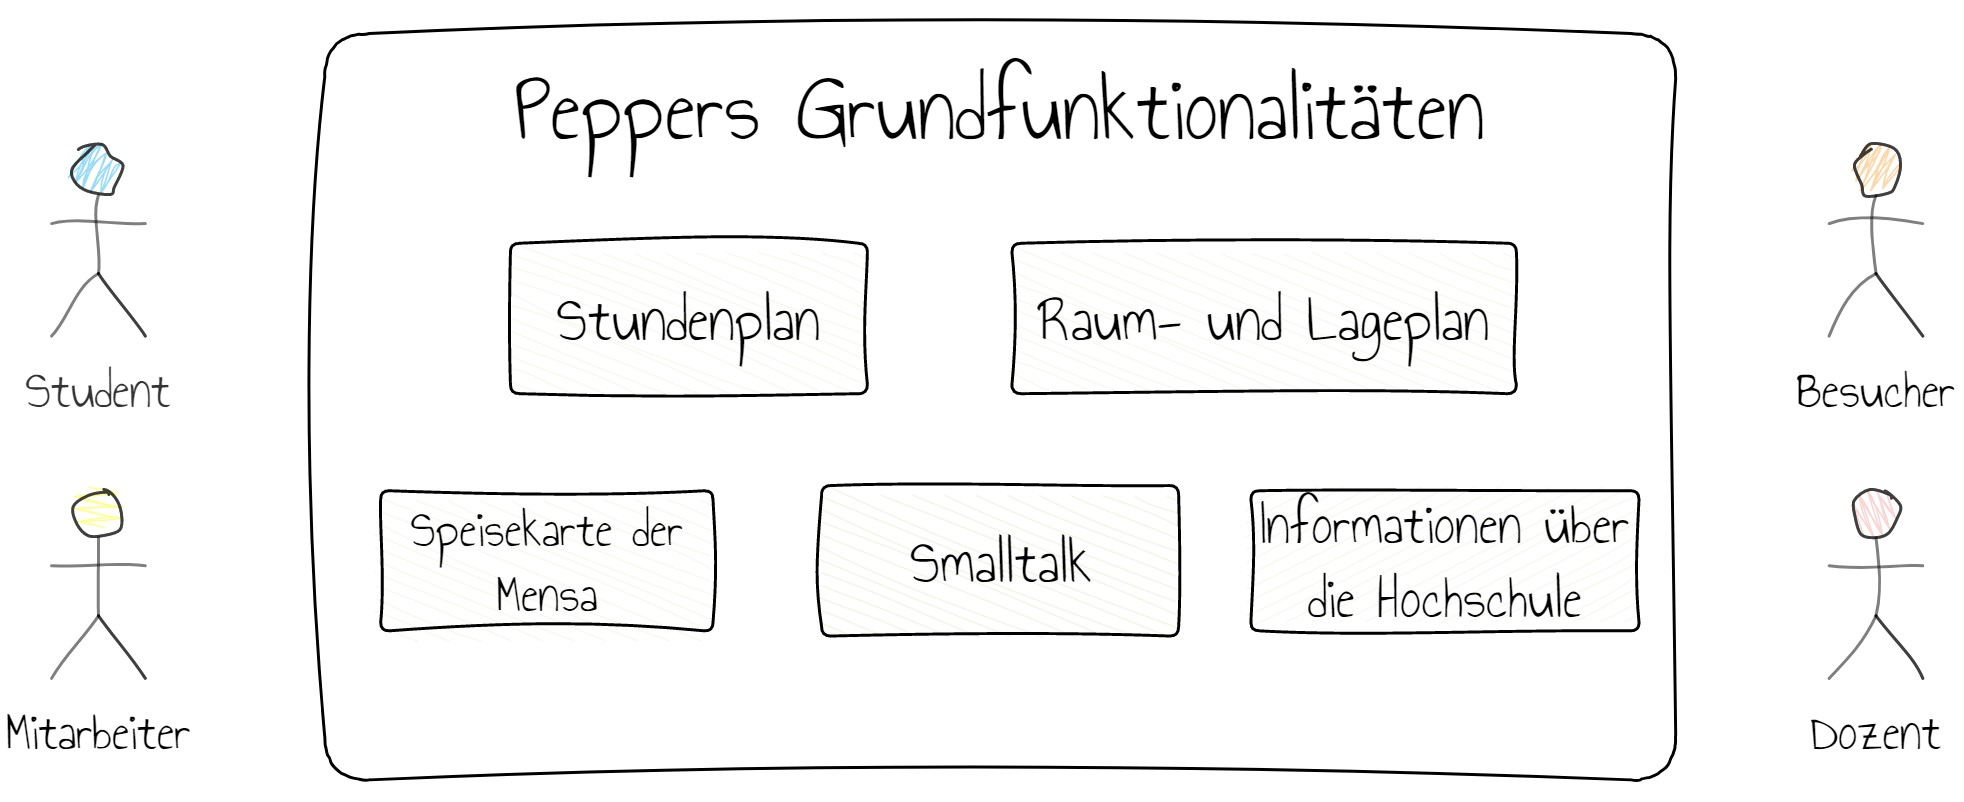
\includegraphics[width=\textwidth]{Figures/pepper-usecase-skizze.jpg}
    \caption{Skizze: Konzeptplanng der Anwendungsfälle}
    \label{fig:integration}
    \centering
\end{figure}

% \begin{figure}[H]
% \includegraphics[width=\textwidth]{}
% \caption{Grundfunktionalitäten}
% \label{fig:skizze}
% \centering
% \end{figure}


In Abb. %\ref{fig:skizze}
ist zu sehen, dass wir folgende Grundfunktionalitäten definiert haben:

\begin{itemize}
    \item Stundenplan
    \item Raum- und Lageplan
    \item Speisekarte der Mensa
    \item Smalltalk
    \item Informationen über die Hochschule
\end{itemize}

Auf Grundlage der diese Grundfunktionalitäten haben wir damit begonnen die Anwendungsfälle weiter zu spezifizieren in dem wir diese in einem Anwendungsfall-Diagramm zusammen getragen haben. 

\begin{figure}[H]
    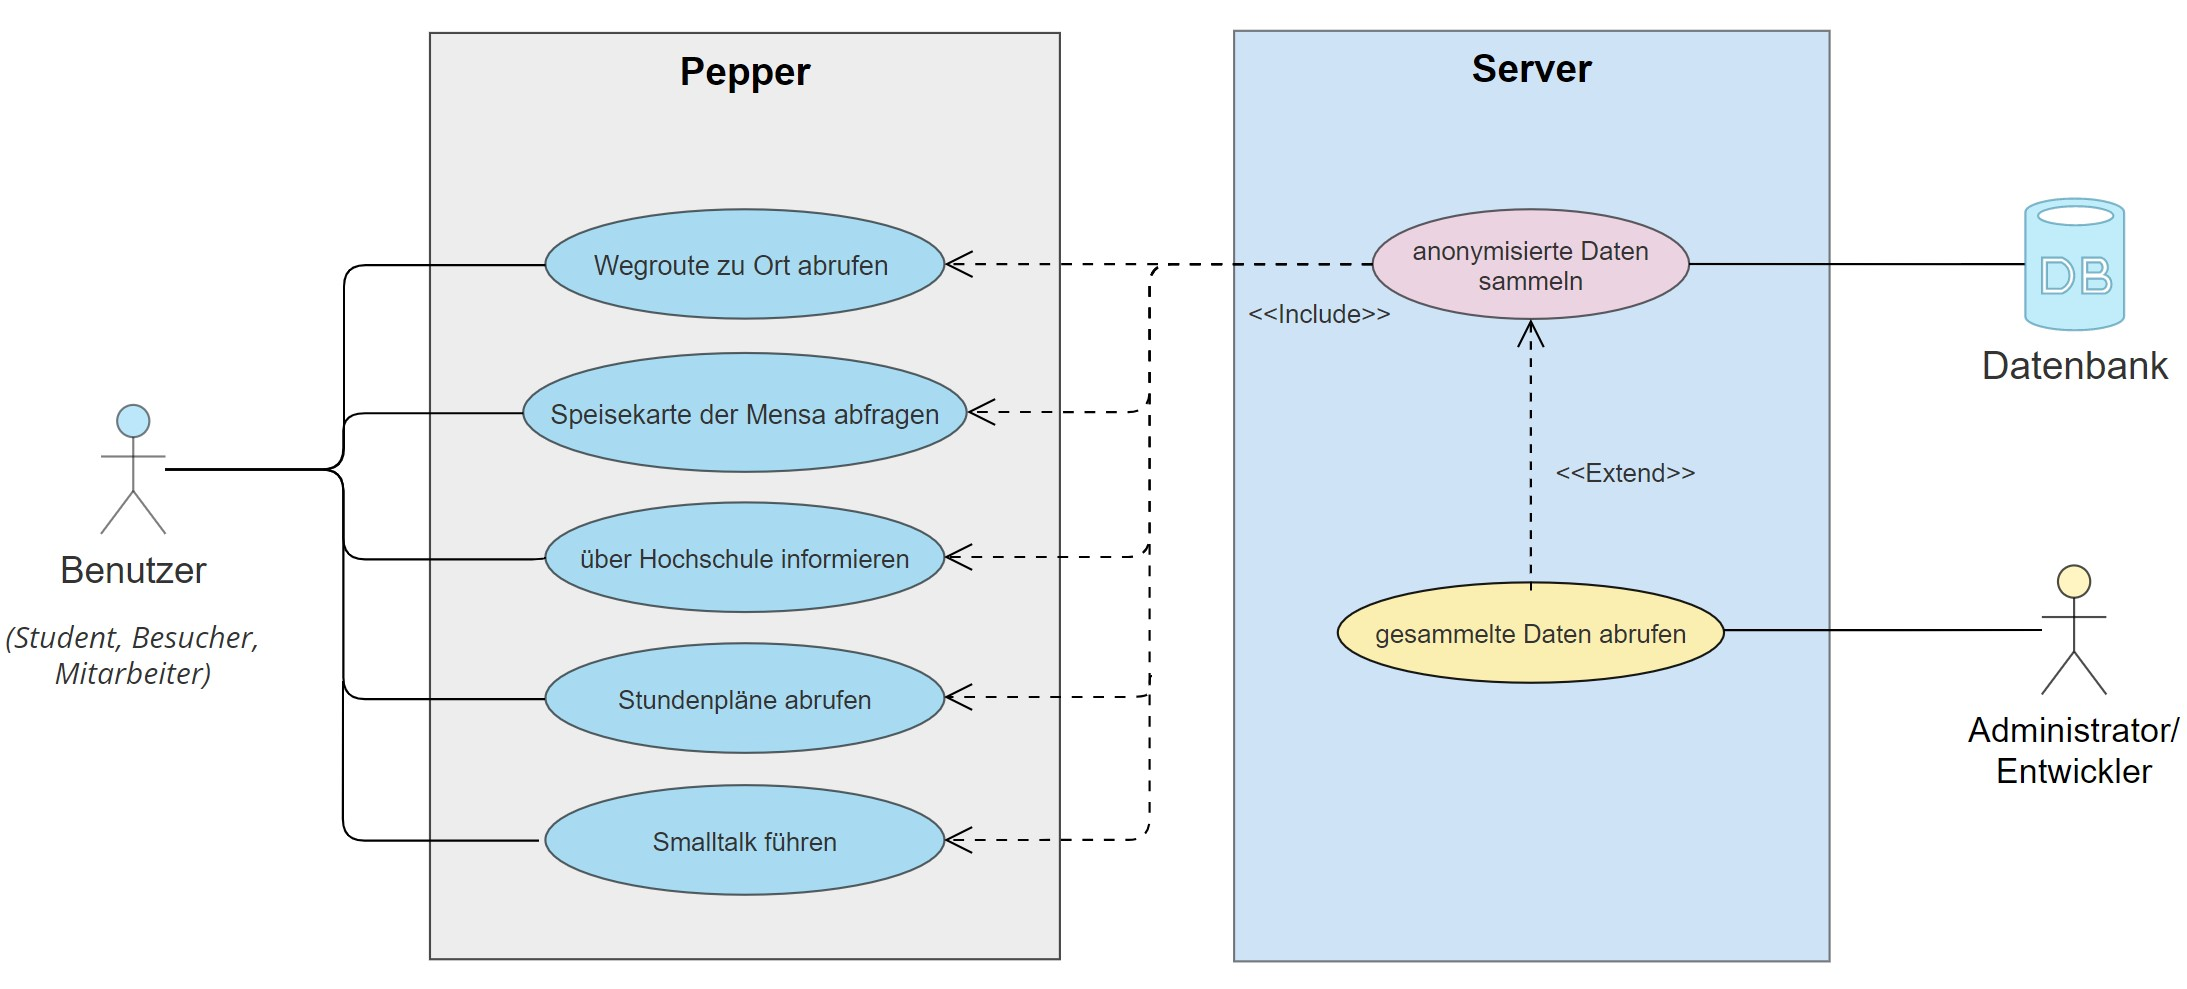
\includegraphics[width=\textwidth]{Figures/use-case-diagram.jpg}
    \caption{Diagramm: Anwendungsfall-Diagramm}
    \label{fig:integration}
    \centering
\end{figure}

Wir haben hierbei die nutzbaren Funktionalitäten für die jeweiligen Akteure der Software voneinander getrennt und in Beziehung zueinander gesetzt. Die Anwendung haben wir in zwei verschiedene Grundsysteme voneinander getrennt. Pepper selbst bietet Funktionalitäten für die Akteure der linken Seite des Diagramms, dies können Studenten, Mitarbeiter, Dozenten oder Besucher der Hochschule sein. Rechts sind die serverseitigen Funktionalitäten der Anwendung darstellt, welche Beispielsweise durch uns Entwickler selbst oder einem zugeteiltem Admin des Systems zur verwendbar sind. Es wäre an dieser Stelle auch denkbar, dass hier an den Daten interessierte Personen der Hochschule, wie beispielsweise Werbeagenturen usw. Zugriff auch diese Funktionalitäten erhalten.

Zudem soll die Interaktion mit Pepper für alle möglich sein. Studierende und Lehrende sollen erfragen können,
wo welche Vorlesung stattfindet, in der Kaffeteria oder Mensa soll sich Pepper mit Gästen unterhalten, Smalltalk führen oder
Empfehlungen für bestimmte Speisen ausgeben. Darüber hinaus wollen wir Pepper das lückenlose Interagieren beibringen, damit er an
besonderen Veranstaltungen, wie dem Tag der offenen Tür oder dem Tag der Informatik, Interessenten Informationen über die Hochschule,
das Leben auf dem Campus, sowie allgemeine Empfehlungen für die Stadt Bremerhaven ausgeben kann.

Die geplante Struktur der Anwendung lässt sich mit der unten dargestellten Abbildung möglichst einfach verdeutlichen. 

\begin{figure}[H]
    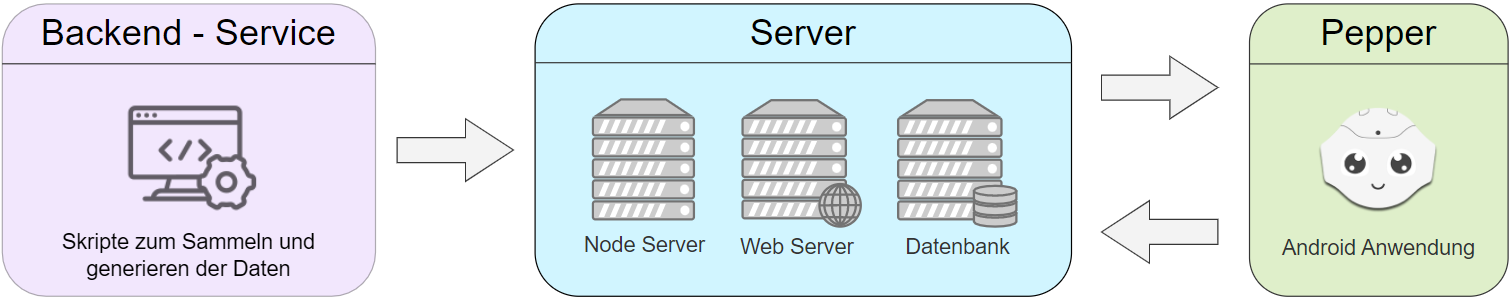
\includegraphics[width=\textwidth]{Figures/anwendungarchitektur.png}
    \caption{Diagramm: Architektur der Anwendung}
    \label{fig:integration}
    \centering
\end{figure}

Die Architektur ist in drei verschiedene Systeme unterteilt, welche in der mit den Pfeilen dargestellten Beziehung zueinander stehen. Hierbei ist der Bereich des Backend-Service ausschließlich dafür da, Daten zu sammeln oder zu generieren, welche dann an den Server gesendet werden. Der Server besteht im groben aus dem Node Server, dem Web Server sowie der Datenbank. Im Gegensatz zu dem Backend-Service steht Pepper mit Server stehen ständig in einem asynchronen Austausch miteinander.

\section{Entwicklungsumgebungen für Pepper}

Um das Verhalten von Pepper zu programmieren, kann entweder die Entwicklungsumgebung Android Studio oder Choregraphe verwendet werden. 
Im Folgenden werden kurz auf die einzelnen Softwares eingehen und erklären, wieso wir uns für Android Studio entschieden haben. 
Anschließend gehen wir noch auf eine weitere Entwicklungsumgebung ein, die aber nicht mehr von Softbanks unterstützt wird.

\subsection{Choregraphe}

Mit der Choregraphe Entwicklungsumgebung können komplexe Verhaltensmuster in Pepper integriert werden, ohne eine Zeile Code zu schreiben. 
Zusätzlich kann das Verhalten aber auch mit der Programmiersprache Python gesteuert werden. Der Choregraphe besitzt mehrer Editoren, 
mit denen sich zum Beispiel Animationen erstellen lassen können oder Gesprächsfunktionen einbinden lassen. Die Software besitzt ebenfalls 
einen Emulator mit einem virtuellen Roboter, wo die Applikation getestet werden kann.
\cite{Choregraphe}

\subsection{Android Studio}

Mit Android Studio können Applikationen für Googles quelloffenes mobiles Betriebssystem entwickelt werden. Sie wurde so konzipiert, dass 
auch Nicht-Programmierer damit arbeiten können, da sie Editoren anbietet, die das Erstellen von Layouts oder Themes vereinfacht. 
Die Software basiert auf IntelliJ IDEA 14 und verwendet somit die Programmiersprachen Java und Kotlin. Beim Erstellen einer neuen 
Applikation kann zwischen diesen beiden Programmiersprachen ausgewählt werden.

Die Software besitzt ihren eigenen SDK Manager, worüber die Pepper SDK heruntergeladen werden kann, um eine Entwicklungsumgebung für Pepper 
zu schaffen. Mit diesen Entwicklungspaketen kommen viele verschiedene Methoden und Funktionen hinzu, worüber sich das Verhalten von Pepper 
steuern und programmieren lässt. Zusätzlich dazu bietet das Pepper SDK einen Emulator an, wo die Applikation auf einem virtuellen Pepper 
getestet werden kann und einen weiteren Editor, mit denen Animationen erstellt werden können. Das Tablet von Pepper kann komplett mit den 
Funktionen und Editoren von Android Studio editiert werden. 

Sowohl Android Studio als auch Choregraphe können bestimmte Komponenten von Pepper nicht ansteuern oder verändern. Hierzu gehört zum 
Beispiel die Kamera von Pepper, da die einzelnen Funktionen wie die Bilderkennung fest verankert sind. Es kann lediglich nur auf die Daten 
zugegriffen werden, die Pepper selber mit seinen Kameras erzeugt.
\cite{Android_Studio}

\subsection{ROS}

Es gab vor ein paar Jahren auch die Möglichkeit, Pepper mit ROS zu entwickeln. 
ROS heißt übersetzt \glqq Robot Operating System \glqq{} und ist somit ein Betriebssystem, das speziell für die Steuerung und Programmierung 
von Robotern entwickelt wurde. Anders als bei Android Studio oder Choregraphe, besitzt man hier jegliche Freiheiten, den Roboter so zu 
programmieren, wie man will. Zum Beispiel hätten wir mit ROS die Möglichkeit gehabt, auf die Kamera oder Sensoren von Pepper zuzugreifen. 
Dies hätte den Vorteil gehabt, dass wir unsere eigene Bild, oder Spracherkennungs-KI für Pepper entwickeln könnten. Softbanks hat sich 
jedoch ab einer früheren Version dazu entschieden, die Kompatibilität und Anbindung mit ROS zu stoppen. Wäre ROS für uns eine Option 
gewesen, hätten wir uns definitiv dafür entschieden. 

\section{Entscheidung}

Wir haben uns dazu entschieden, Android Studio als Entwicklungsumgebung zu verwenden, da wir mit der Pepper SDK eine Vielzahl an 
Möglichkeiten besitzen, Pepper für jede Situation anzupassen. Außerdem wurde es uns auch von den Masterstudenten empfohlen und wir konnten 
deren Applikation als Referenz verwenden. Für unsere Applikation haben wir uns entschieden, Java statt Kotlin als Programmiersprache zu 
verwenden, da wir damit die meisten Erfahrungen gemacht haben. 

\section{Hard- und Softwarespezifikationen}
%Da Peppers Tablet auf Android basiert, liegt es auf der Hand, Android Studio als Entwicklungsumgebung zu benutzen. Der
Einfachheit halber, ist nachfolgend eine Tabelle, welche die von uns für die Pepper Anwendung benutzte Software mit den
entsprechenden Versionsnummern auflsitet.

\begin{table}[H]
    \caption{Hard- und Softwarespezifikationen}
    \label{table}
    \setlength{\tabcolsep}{3pt}
    \begin{tabular}{|p{100pt}|p{120pt}|p{180pt}|}
        \hline
        Software / Tool & Version / Spezifikation     & Beschreibung                                                                     \\
        \hline\hline
        Android Studio  & Arctic Fox 2020.3.1 Patch 4 & IDE der IntelliJ Plattform                                                       \\
        \hline
        Gradle          & 7.0.3                       & Build Tool                                                                       \\
        \hline
        Android SDK     & 12                          & Android Framework                                                                \\
        \hline
        Pepper API      & v1.9  API 23                & Entwicklungstools für Pepper mit Emulator, Deploy und Debug Funktion             \\
        \hline
        Android API SDK & 31                          & Framework zum Verbinden und Installieren von Software auf Geräten mit Android OS \\
        \hline
        Java SDK        & 1.8                         & Basis der Programmiersprache Java und dessen Grundfunktionalitäten               \\
        \hline
        \multicolumn{3}{p{380pt}}{Mit abwichenden Versionen kann es zu Kompatibilitätsproblemen kommen.}
    \end{tabular}
    \label{tab1}
\end{table}

%Um unsere Software von zu Hause aus zu testen, nutzen wir den Build-In Emulator, welcher bei der installation
%der Pepper API in Android Studio integriert wird. Hiermit ist es möglich die sprachliche Kommunikation zwischen
%Pepper und dem Anwender, sowie die Aus- und Eingaben auf dem Tablet zu testen.

Der Roboter Pepper selbst, ist XXX groß, wurde am XXX von XXX gekauft und ist seit XXX im Besitz der Hochschule
und läuft derzeit mit der Version XXX.

%\section{Implementierung}

%\textbf{hier muss auch erwähnt werden, dass pepper selbst das alter, stimmung und geschlecht erkennt}
% \begin{figure}[H]
% \includegraphics[width=\textwidth]{bannerNmenu}
% \caption{Banner und Menülesite im angemeldeten Zustand als Admin}
% \label{fig:menu}
% \centering
% \end{figure}

% In der Menüleiste werden je nach Anmeldestatus des Nutzers, andere Unterpunkte dargestellt. Nicht registrierte Nutzer haben keine Möglichkeit, ein Portfolio einzusehen oder auf unsere exklusive \grqq{}Gamble\grqq{} Seite zu gelangen. Des Weiteren beinhaltet die Menüleiste alle relevanten Links und Weiterleitungen unserer Website, sowie ein animiertes Widget von \href{https://de.tradingview.com/}{TradingView}, welches aktuelle Kursdaten zu ausgewählten Wertpapieren in Dauerschleife anzeigt. Das Logo unserer Website wurde von Leonhard T. Schwertfeger \cite{mygainlogo} erstellt und zur Verfügung gestellt.

% Zu Anfang des Projektes haben wir auf der Startseite, um sie etwas lebhafter zu gestalten, mehrere Widgets von \href{https://de.tradingview.com/ }{TradingView} mittels JavaScript eingebunden, jedoch haben wir im Laufe der Zeit gemerkt, dass es gar nicht so schwierig ist, Kursdaten wie der Öffnungs- und Schlusskurs oder auch Tageshöchst- und Tiefstwerte abzubilden, wenn man die nötigen Datensätze besitzt. Die Herkunft der bei uns benutzten Daten besprechen wir in Kapitel \ref{sec:MyGain-Trade} - Trade.

% Da wir unseren Kunden eine schnelle Einsicht in unser Angebot ermöglichen wollen, ist der iFrame so eingestellt, dass er standardmäßig die \code{home.php} Seite anzeigt, welche in zwei Bereiche eingeteilt ist. Drei Viertel der Seite nimmt eine tabellarische Übersicht aller bei uns handelbaren Assets ein. Diese beinhaltet alle relevanten Kursdaten wie \grqq{}Open\grqq{}, \grqq{}Close\grqq{}, \grqq{}High / Low\grqq{} und das Volumen des Assets. Diese Daten beziehen sich auf den Zeitraum von einen Tag. Zudem besteht die Möglichkeit der direkten Weiterleitung auf die Trade Seite, sofern eines der angebotenen Wertpapiere angeklickt wird.\\

% \begin{figure}[H]
% \includegraphics[width=\textwidth]{home}
% \caption{MyGain - Home Seite}
% \label{fig:homesite}
% \centering
% \end{figure}

% (Abb. \ref{fig:homesite}) Im rechten Viertel der Seite haben wir eine kleine Begrüßungsformel stehen, um Besuchern wissen zu lassen, dass hier auch Menschen am arbeiten sind. Des weiteren wird man dort, sofern man eingeloggt ist, mit einem \grqq{}Moin \code{<username>}!\grqq{} empfangen, um unseren Kunden so nah wie möglich zu sein. Als kleines Gimmick haben wir einen Besucherzähler eingebaut, der die Anzahl der Seitenaufrufe unserer Index Seite zählt. \\
 % Konzept: Pepper app

\chapter{Pepper App; Anwendungsfall - Hochschule}
\label{sec:anwendungsfall-hochschule}
\lhead{Kapitel 4. \emph{Anwendungsfall - Hochschule}}

\section{Die Vorüberlegungen}
Nachdem wir uns darauf geeinigt haben, mindestens einen Anwendungsfall für den Roboter Pepper zu entwickeln,
und sich dieser auf den Alltag an der Hochschule Bremerhaven beziehen soll, haben wir uns damit konfrontiert gesehen,
uns Gedanken darüber zu machen, wie genau eine Interaktion zwischen einem Studenten oder einer Lehrkraft und dem Roboter
stattfinden kann. Aufgrund der den aktuellen Beschlüssen der Regierung ist das Leben auf dem Campus fast zum Stillstand gekommen,
wodurch sich für Pepper wenige Einsatzgebiete ergeben. Wir gehen jedoch davon aus, zu einer neuen Normalität zurück zu gekangen,
und werden Pepper dahingehend vorbereiten.

Folgende Fragen sind für uns zentral:
\begin{itemize}
    \item Wie sieht der Alltag auf dem Campus aus?
    \item Wann soll Pepper mit wem interagieren?
    \item Welche Funktionalitäten wollen wir implementieren?
    \item Wo setzen wir welche Werkzeuge ein?
    \item Wo fangen wir an?
\end{itemize}

Wir sind dann ziemlich schnell darauf gekommen, dass wir eine klare Struktur benötigen,
um unsere Aufgaben und Ziele klar zu definieren. Daraufhin ist folgende Skizze entstanden,
welche grob die Hauptfunktionalitäten unseres Projektes festhält:
\begin{center}
    \textbf{HIER WIRKLICH EINE SKIZZE ANFERTIGEN}
\end{center}

% \begin{figure}[H]
% \includegraphics[width=\textwidth]{}
% \caption{Grundfunktionalitäten}
% \label{fig:skizze}
% \centering
% \end{figure}


In Abb. %\ref{fig:skizze}
ist zu sehen, dass wir folgende Grundfunktionalitäten definiert haben:

\begin{itemize}
    \item Stundenplan
    \item Raum- und Lageplan
    \item Speisekarte der Mensa
    \item Smalltalk
\end{itemize}

Zudem soll die Interaktion mit Pepper für alle möglich sein. Studierende und Lehrende sollen erfragen können,
wo welche Vorlesung stattfindet, in der Kaffeteria oder Mensa soll sich Pepper mit Gästen unterhalten, Smalltalk führen oder
Empfehlungen für bestimmte Speisen ausgeben. Darüber hinaus wollen wir Pepper das lückenlose Interagieren beibringen, damit er an
besonderen Veranstaltungen, wie dem Tag der offenen Tür oder dem Tag der Informatik, Interessenten Informationen über die Hochschule,
das Leben auf dem Campus, sowie allgemeine Empfehlungen für die Stadt Bremerhaven ausgeben kann.

\section{Hard- und Softwarespezifikationen}
Da Peppers Tablet auf Android basiert, liegt es auf der Hand, Android Studio als Entwicklungsumgebung zu benutzen. Der
Einfachheit halber, ist nachfolgend eine Tabelle, welche die von uns für die Pepper Anwendung benutzte Software mit den
entsprechenden Versionsnummern auflsitet.

\begin{table}[H]
    \caption{Hard- und Softwarespezifikationen}
    \label{table}
    \setlength{\tabcolsep}{3pt}
    \begin{tabular}{|p{100pt}|p{120pt}|p{180pt}|}
        \hline
        Software / Tool & Version / Spezifikation     & Beschreibung                                                                     \\
        \hline\hline
        Android Studio  & Arctic Fox 2020.3.1 Patch 4 & IDE der IntelliJ Plattform                                                       \\
        \hline
        Gradle          & 7.0.3                       & Build Tool                                                                       \\
        \hline
        Android SDK     & 12                          & Android Framework                                                                \\
        \hline
        Pepper API      & v1.9  API 23                & Entwicklungstools für Pepper mit Emulator, Deploy und Debug Funktion             \\
        \hline
        Android API SDK & 31                          & Framework zum Verbinden und Installieren von Software auf Geräten mit Android OS \\
        \hline
        Java SDK        & 1.8                         & Basis der Programmiersprache Java und dessen Grundfunktionalitäten               \\
        \hline
        \multicolumn{3}{p{380pt}}{Mit abwichenden Versionen kann es zu Kompatibilitätsproblemen kommen.}
    \end{tabular}
    \label{tab1}
\end{table}

%Um unsere Software von zu Hause aus zu testen, nutzen wir den Build-In Emulator, welcher bei der installation
%der Pepper API in Android Studio integriert wird. Hiermit ist es möglich die sprachliche Kommunikation zwischen
%Pepper und dem Anwender, sowie die Aus- und Eingaben auf dem Tablet zu testen.

Der Roboter Pepper selbst, ist XXX groß, wurde am XXX von XXX gekauft und ist seit XXX im Besitz der Hochschule
und läuft derzeit mit der Version XXX.

\section{Implementierung}


% \begin{figure}[H]
% \includegraphics[width=\textwidth]{bannerNmenu}
% \caption{Banner und Menülesite im angemeldeten Zustand als Admin}
% \label{fig:menu}
% \centering
% \end{figure}

% In der Menüleiste werden je nach Anmeldestatus des Nutzers, andere Unterpunkte dargestellt. Nicht registrierte Nutzer haben keine Möglichkeit, ein Portfolio einzusehen oder auf unsere exklusive \grqq{}Gamble\grqq{} Seite zu gelangen. Des Weiteren beinhaltet die Menüleiste alle relevanten Links und Weiterleitungen unserer Website, sowie ein animiertes Widget von \href{https://de.tradingview.com/}{TradingView}, welches aktuelle Kursdaten zu ausgewählten Wertpapieren in Dauerschleife anzeigt. Das Logo unserer Website wurde von Leonhard T. Schwertfeger \cite{mygainlogo} erstellt und zur Verfügung gestellt.

% Zu Anfang des Projektes haben wir auf der Startseite, um sie etwas lebhafter zu gestalten, mehrere Widgets von \href{https://de.tradingview.com/ }{TradingView} mittels JavaScript eingebunden, jedoch haben wir im Laufe der Zeit gemerkt, dass es gar nicht so schwierig ist, Kursdaten wie der Öffnungs- und Schlusskurs oder auch Tageshöchst- und Tiefstwerte abzubilden, wenn man die nötigen Datensätze besitzt. Die Herkunft der bei uns benutzten Daten besprechen wir in Kapitel \ref{sec:MyGain-Trade} - Trade.

% Da wir unseren Kunden eine schnelle Einsicht in unser Angebot ermöglichen wollen, ist der iFrame so eingestellt, dass er standardmäßig die \code{home.php} Seite anzeigt, welche in zwei Bereiche eingeteilt ist. Drei Viertel der Seite nimmt eine tabellarische Übersicht aller bei uns handelbaren Assets ein. Diese beinhaltet alle relevanten Kursdaten wie \grqq{}Open\grqq{}, \grqq{}Close\grqq{}, \grqq{}High / Low\grqq{} und das Volumen des Assets. Diese Daten beziehen sich auf den Zeitraum von einen Tag. Zudem besteht die Möglichkeit der direkten Weiterleitung auf die Trade Seite, sofern eines der angebotenen Wertpapiere angeklickt wird.\\

% \begin{figure}[H]
% \includegraphics[width=\textwidth]{home}
% \caption{MyGain - Home Seite}
% \label{fig:homesite}
% \centering
% \end{figure}

% (Abb. \ref{fig:homesite}) Im rechten Viertel der Seite haben wir eine kleine Begrüßungsformel stehen, um Besuchern wissen zu lassen, dass hier auch Menschen am arbeiten sind. Des weiteren wird man dort, sofern man eingeloggt ist, mit einem \grqq{}Moin \code{<username>}!\grqq{} empfangen, um unseren Kunden so nah wie möglich zu sein. Als kleines Gimmick haben wir einen Besucherzähler eingebaut, der die Anzahl der Seitenaufrufe unserer Index Seite zählt. \\
 % Implementierung: Pepper App

\newcommand{\chapterpepperusecase}{Kapitel 6. }

\chapter{Implementierung: Anwendungsfälle}
\label{sec:Pepper_Anwendungsfaelle}
\lhead{\chapterpepperusecase \emph{Implementierung der Anwendungsfälle}}

Im Folgenden werden wir auf die Implementierung unserer Anwendungsfälle eingehen. Hierbei gehen wir zuerst auf die Planung und anschließend auf die Bereitstellung der Daten in unserem Server und in externe Scripts ein. Anschließend erläutern wir die Implementation und Weiterverarbeitung der einzelnen Anwendungsfälle in Android Studio.\\

\section{Mensa}

Der Anwendungsfall für die Mensa ist in zwei Teile aufgeteilt. Der erste Teil ist das Anzeigen des Mensaplans auf dem Tablet von Pepper. Sollte der Anwender explizit nach dem Mensaplan fragen, muss Pepper in der Lage sein, eine Übersicht des Mensaplans der aktuellen Woche anzuzeigen. 
Der zweite Teil ist das verbale Beschreiben der Mensaangebote. Hierbei soll Pepper für jeden Wochentag erzählen können, welche Angebote in der Mensa zurzeit zur Verfügung stehen. Die Mensa der Hochschule Bremerhaven bietet jeden Wochentag immer zwei Angebote an. Das zweite Angebot ist dabei immer vegetarisch. Pepper muss dementsprechend in der Lage sein, beide Angebote beschreiben zu können. 

Um die verschiedenen Daten über die Mensa Angebote abrufen zu können, verwenden wir unseren Server, der diese Daten bereitstellt. Der Server bekommt diese Daten aus einem externen Python Script.\\

\subsection{Script um Mensadaten aufzurufen}
\label{sec:pyMensa}

Um die Daten auf dem Server anzeigen zu lassen, wird ein Python Script verwendet, dass sich diese Daten aus der offiziellen Hochschule Bremerhaven Mensa Webseite zieht. 

Webseite: \url{https://www.stw-bremen.de/de/cafeteria/bremerhaven}

Auf dieser Webseite befinden sich die aktuellen Angebote für die nächsten fünf Tage in einer Tabelle und den aktuellen- sowie nächsten Wochenplan im PDF-Format. Mit dem Script werden die einzelnen Daten aus der Webseite gelesen und als JSON gespeichert. Das Lesen der Daten aus der Webseite wird mit Hilfe des Frameworks \verb|BeautifulSoup| durchgeführt. Dieses Framework erlaubt es, XML- und HTML-Dokumente zu \verb|parsen|.\\

\begin{lstlisting}[language=Python]
menulist = soup.select('tbody')

menu, offer1, offer2 = {}, [], []
day: [str] = [
    'Montag', 'Dienstag', 'Mittwoch', 'Donnerstag', 'Freitag'
    ]
\end{lstlisting}

Die Mensa Angebote befinden sich auf der Webseite in einer Tabelle, weshalb wir auf alle \verb|tbody|-Elemente mit der Funktion \verb|soup.select| zugreifen. Diese werden als Array in die Variable \verb|menulist| initialisiert. Anschließend werden die Variablen deklariert, aus denen später der JSON string entstehen soll. \\

\begin{lstlisting}[language=Python]
for i in range(10):
    tmp = (str(menulist[i]).split('description">',1)[1]).rsplit
    ("</td><td",2)[0]
    tmp = tmp.replace('\n',').replace('\r',').replace('a1',')
    .replace('amp;',')
    tmp = re.sub('<sup>.*?</sup>', |, tmp)
    if(i%2==0): offer1.append(tmp)
    else: offer2.append(tmp)
    menu'"day'], menu['offer1'], menu['offer2'] = day, offer1, offer2

with open(folder_location+"mensadata.json", "w+") as f:
    json.dump(menu, f, ensure_ascii=False)
\end{lstlisting}

Da sich die Daten in den \verb|tbody|-Elementen schwer lesen lassen, werden diese mit mehreren \verb|split| und \verb|replace| Funktionen in lesbare Mensa Angebote umgeformt und in den einzelnen Variablen eingefügt. Die If-Bedingung wird verwendet, um das erste- und zweite Angebot voneinander zu trennen. Anschließend wird das \verb|menu| Objekt mit den keys \verb|day|, \verb|offer1| und \verb|offer2| und den Values der jeweiligen Arrays initialisiert.
Zum Schluss wird das \verb|menu| Objekt in JSON mit der \verb|json.dump| Funktion umgewandelt.

Um den aktuellen Wochenplan im Script herunterzuladen und weiterzuverarbeiten, wird die Programmbibliothek Poppler vorausgesetzt. Poppler wird in Unix-ähnlichen Betriebssystemen dazu verwendet, PDF-Dateien anzuzeigen.\\

\begin{lstlisting}[language=Python]
response = requests.get(url)
soup = BeautifulSoup(response.text, 'html.parser')
menucard = ((str(soup.select("a[href$='/print']")[0])
.rsplit(' target',1)[0]).split('href=',1)[1])
.replace('"',|)
urllib.request.urlretrieve(menucard, f'{folder_location}Mensaplan.pdf')
\end{lstlisting}

Mit den ersten beiden Zeilen des Codes wird der komplette HTML-Inhalt der Webseite in die Variable \verb|soup| initialisiert. Da wir die URL des aktuellen Wochenplans benötigen, muss dieser aus dem HTML Code gelesen werden. Der Standort dieser URL ist im HTML Code fest verankert, weswegen wir mit Hilfe von \verb|soup.select|, die URL herausfiltern und mit mehreren \verb|split| und \verb|replace| Funktionen zu einer gültigen URL umformen können. Dieser Zwischenschritt ist nötig, da sich die URL jede Woche ändert. Anschließend wird die URL aufgerufen und als \verb|Mensaplan.pdf| abgespeichert.\\

\begin{lstlisting}[language=Python]
img = convert_from_path(f'{folder_location}Mensaplan.pdf', 500)[0]

area = (0, 200, 4134, 2800) # R T L B
cropped_img = img.crop(area)

area = (0, 5200, 4134, 5800)
cropped_img2 = img.crop(area)
mergeImgs([cropped_img, cropped_img2])
.save(folder_location+'images/mensaplan.png', 'JPEG')
\end{lstlisting}

Im nächsten Schritt wird mit der Funktion \verb|convert_from_path| das PDF in ein Bildformat konvertiert und in die Variable \verb|img| installiert. Hierfür wird das Framework \verb|pdf2image| verwendet, das vorab mit \verb|pip| installiert werden muss. 

Nun ist das Bild jedoch im Hochformat und kann sehr schlecht auf dem Tablet von Pepper angezeigt werden. Somit haben wir das Bild in zwei Teile geschnitten und im Querformat zusammengefügt (vgl. Abb. \ref{fig:Mensaplan}). Um das Bild zu schneiden, haben wir das Framework \verb|PIL| verwendet. Nun kann genau angegeben werden, wie das Bild geschnitten werden soll. In der Variable \verb|area| haben wir jeweils immer vordefiniert, wie weit das Bild in welcher Richtung ausgeschnitten werden soll. Die Reihenfolge der Richtungen lautet wie folgt: 
(rechts oben links unten) (0, 200, 4134, 2800)

Zuerst haben wir den oberen Teil des Mensaplans ausgeschnitten, der die einzelnen Angebote enthält und anschließend die Legende, die sich im unteren Bereich der PDF befindet. 

Nun müssen beide Bilder zusammengefügt werden. Dies wurde in der Methode \verb|mergeImgs| durchgeführt.\\


\begin{lstlisting}[language=Python]
def mergeImgs(imgs):
    min_img_width = min(i.width for i in imgs)
    
    total_height = 0
    for i, img in enumerate(imgs):
    
    if(img.width > min_img_width):
        imgs[i] = img.resize((min_img_width, int(img.height / 
        img.width * min_img_width)), Image.ANTIALIAS)
    total_height += imgs[i].height
    
    img_merge = Image.new(imgs[0].mode, (min_img_width, total_height))
    y = 0
    for img in imgs:
        img_merge.paste(img, (0, y))
    
        y += img.height
    return img_merge
\end{lstlisting}

In dieser Funktion wird zuerst die Breite und Höhe des neu zusammengefügten Bildes ermittelt. Sollten die beiden Bilder eine unterschiedliche Breite besitzen, wird das breiteste Bild verkleinert. Dies geschieht in der For-Schleife, wo jedes einzelne Bild überprüft wird. 
Anschließend wir ein neues \verb|img_merge| Objekt erzeugt, das mit der minimalsten Breite und addierten Höhe der beiden Bilder initialisiert wird. Zum Schluss werden die beiden Bilder in das Objekt eingefügt und heruntergeladen.

\begin{figure}[H]
    \centering
    \includegraphics[width=15cm]{Figures/AppChapter/mensa_3.png}
    \caption{Mensaplan - cropped}
    \label{fig:Mensaplan}
    \centering
\end{figure}

\subsection{Weiterleitung zum NodeJS Server}

Das Script (vgl. Abschnitt \ref{sec:pyMensa}) befindet sich auf dem Hopper und wird mit \verb|crontab| jeden Montag einmal ausgeführt. Es ist wichtig, dass das Script nur jeden Montag ausgeführt wird, da die Mensa Angebote nur für die nächsten fünf Tage zur Verfügung kann. Sollte das Script zum Beispiel an einem Mittwoch ausgeführt werden, so würden die Tage Montag und Dienstag fehlen.\\

\begin{lstlisting}[language=Bash]
    # m h dom mon dow command
    0 0 * * 1 /usr/bin/python3 ~/getMensaPlan.py
\end{lstlisting}

Das erzeugte JSON Objekt und das zugeschnittene Bild des Mensaplans werden anschließend in den \verb|static| Ordner vom Node Server eingefügt.

\subsection{Bereitstellen der Mensadaten auf dem Server}

Mit dem folgenden Code werden die Daten aus den jeweiligen “/static” Ordnern an die Webseite gesendet:\\

\begin{lstlisting}[language=Java]
router.get('/docker-hbv-kms-http/api/v1/mensadata', (req, res) => {
    const filePath = `${__dirname}/../static/data/mensadata.json`;
    const jsonData = JSON.parse(fs.readFileSync(filePath, 'latin1'));
    res.send(jsonData);
});

router.get('/docker-hbv-kms-http/api/v1/mensadata/img', (req, res) => {
    const filePath = `${__dirname}/../static/images/mensaplan.png`;
    const img = fs.readFileSync(filePath);
    res.writeHead(200, {
        'Content-Type': 'image/png'
    });
    res.end(img, 'binary');
});    
\end{lstlisting}

(vgl. Abb. \ref{fig:mensaapi}) In folgendem Pfad befindet sich nun unser JSON Objekt, mit allen Mensaangeboten der aktuellen Woche.\\
\url{https://informatik.hs-bremerhaven.de/docker-hbv-kms-http/api/v1/mensadata}
\\
\begin{figure}[H]
    \centering
    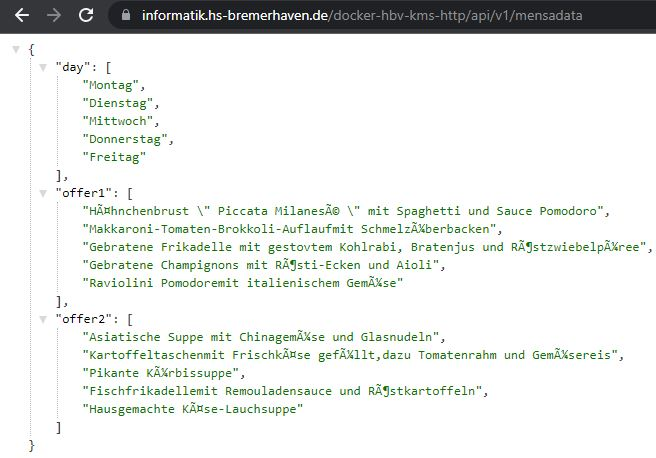
\includegraphics[width=13cm]{Figures/AppChapter/mensa_5.JPG}
    \caption{Mensadaten - API}
    \label{fig:mensaapi}
    \centering
\end{figure}

Der aktuelle Wochenplan ist in png-Format unter folgendem Link erreichbar:\\
\url{https://informatik.hs-bremerhaven.de/docker-hbv-kms-http/api/v1/mensadata/img}\\


\subsection{Anzeigen der Mensadaten in Android Studio}

Wie bereits erwähnt, soll Pepper mit Hilfe von Sprache in der Lage sein, den Mensaplan auf sein Tablet anzuzeigen und Informationen über die verschiedenen Angebote jedes Wochentags zu geben. Um sich den Mensaplan anzeigen zu lassen, haben wir zuerst ein neues Gesprächsthema in unserem Haupt-Topic erstellt. \\

\begin{lstlisting}
u:(["Ich hab{e} hunger" "Zeig {mir} {den} Mensaplan"] ) 
^execute(VariableExecutor, qiVariableMensa, Plan) Hier hast du eine 
Uebersicht ueber den Mensaplan
\end{lstlisting}

Sobald der Anwender nach dem Mensaplan fragt, wird die \verb|runWith| Methode mit den Parametern \verb|qiVariableMensa|
und \verb|Plan| in der \verb|VariableExecutor| Klasse aufgerufen.\\

\begin{lstlisting}[language=Python]
case('qiVariableMensa'):
String day = params.get(1);
if(day.equals('Plan')){
    ...
}
\end{lstlisting}

In dieser Methode wird anschließend nach dem switch 
case \verb|qiVariableMensa| gesucht. Da wir einen zweiten Mensaanwendungsfall besitzen, müssen wir diese beiden Fälle  voneinander unterscheiden können. Aus diesem Grund wurde ein weiterer String Parameter mit dem Namen \verb|Plan| mitgegeben,  um über einer If-Bedingung diese beiden Fälle zu trennen. Nun gibt es mehrere Möglichkeiten, das Bild auf dem Tablet von Pepper anzeigen zu lassen. Die einfachste Methode wäre über den Webviewer. Hierfür hätten wir lediglich die URL benötigt, um die Webseite mit dem Bild auf dem  Tablet anzeigen zu lassen. Die Bildgröße des Mensaplans besaß jedoch eine viel zu große Auflösung (3200 x 4134 px), sodass nur ein Teil des Bildes auf dem Tablet angezeigt werden konnte. Auf dem Node Server oder in Android Studio könnte die Auflösung theoretisch manuell umgestellt werden, was wir jedoch vermeiden wollen. 

Wir haben uns anschließend für eine andere Lösung entschieden, wo das Bild in Android Studio als Bitmap vom Node Server heruntergeladen wird. Eine Bitmap ist eine Zahlenmatrix von einem Bild, wo jeder Pixel die jeweiligen Farbinformationen enthält.\\


\begin{lstlisting}[language=Java]
String url_str = "https://informatik.hs-bremerhaven.de/
docker-hbv-kms-http/api/v1/mensadata/img";
InputStream srt = new URL(url_str).openStream();
final Bitmap bitmap = BitmapFactory.decodeStream(srt);
    
ma.runOnUiThread(() -> {
    ma.setContentView(R.layout.mensa_layout);
    ImageView imageView = (ImageView) ma.findViewById(R.id.iMensa);
    imageView.setImageBitmap(bitmap);
});
\end{lstlisting}

In diesem Code wird das Bild in einen InputStream initialisiert. Ein InputStream ist eine Folge von Bytes, womit sich Daten lesen 
lassen können. Der InputStream wird mithilfe der \verb|BitmapFactory.decodeStream| Funktion in eine Bitmap umgewandelt. 
Anschließend kann eine Imageview mittels der Id mit der Bitmap initialisiert werden. 

Nun kann Pepper auf die Frage ``Zeig mir den Mensaplan'' ein Bild von dem aktuellen Mensaplan auf sein Tablet zeigen. \\

\begin{figure}[H]
    \centering
    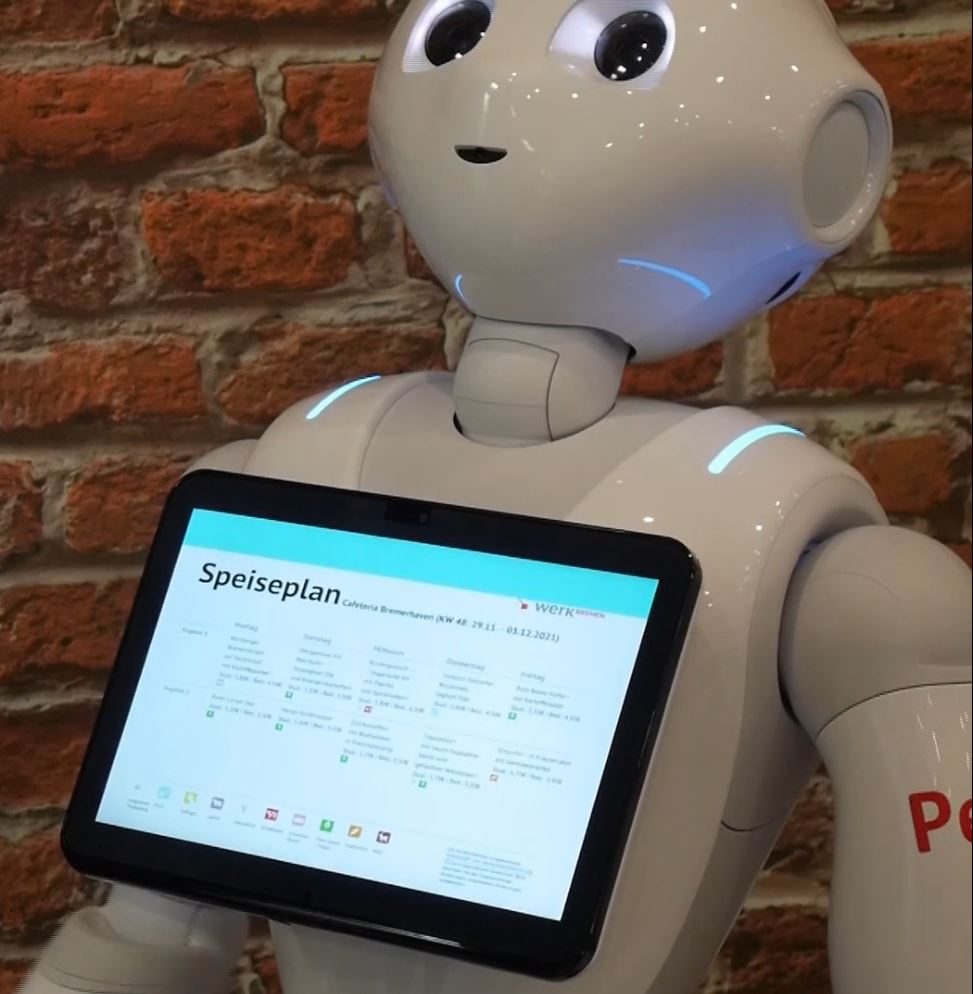
\includegraphics[width=6cm]{Figures/AppChapter/rx2.JPG}
    \caption{Mensaplan auf Hopper}
    \label{fig:mensaplanPepper}
    \centering
\end{figure}

Als Nächstes wird ein weiteres Gesprächsthema erstellt, dass Pepper erlaubt, auch verbal Informationen über die Mensa Angebote zu geben.\\

\begin{lstlisting}
concept:(week) [Montag Dienstag Mittwoch Donnerstag 
Freitag Heute Morgen Uebermorgen]

u:({was} {gibt{s}} {es} {zu} essen {am} _[~week]) $day=$1 
^execute(VariableExecutor, qiVariableMensa, $day) $day gibt 
es entweder $qiVariableMensa

u:({was} {gibt{s}} {es} {am} _[~week] {zu} essen) $day=$1 
^execute(VariableExecutor, qiVariableMensa, $day) $day gibt 
es entweder $qiVariableMensa
\end{lstlisting}

Hier wird die Variable \verb|day| mit dem Wochentag in  \verb|_[~week]| initialisiert, dass in der Frage genannt wurde. Wenn der Anwender zum Beispiel fragt: ``Was gibt es am Mittwoch zu essen'', wird Mittwoch in die Variable \verb|day| initialisiert. In dem Konzept wurden nicht nur Wochentage, sonder auch Wöter wie Heute, Morgen und Übermorgen hinzugefügt. Somit kann der Anwender auch fragen, was es zum Beispiel morgen zu essen gibt. Anschließend wird wieder die \verb|runWith| Methode aufgerufen mit den Parameter \verb|qiVariableMensa| und dem Wochentag, der genannt wurde. In der VariableExecutor Klasse wird nun die Antwort vorbereitet, die Pepper zu der Frage geben soll. Hierfür wird die \verb|getOffer| Methode in 
der HelperCollection Klasse aufgerufen.\\

\begin{lstlisting}[language=Java]
HttpURLConnection con = getConnection("https://informatik.
hs-bremerhaven.de/docker-hbv-kms-http/api/v1mensadata");

BufferedReader in = new BufferedReader(new InputStreamReader(
    con.getInputStream()));
String inputLine;
StringBuffer response = new StringBuffer();
while ((inputLine = in.readLine()) != null) response.append(inputLine); 
in.close();

JSONObject myResponse = new JSONObject(response.toString());
String tmp = myResponse.getString("offer1");
String [] offer1 = tmp.split("\",\"", -1);
tmp = myResponse.getString("offer2");
String [] offer2 = tmp.split("\",\"", -1); 
\end{lstlisting}

Zuerst werden die Daten aus dem Server aufgerufen und mithilfe des \verb|BufferedReader| in das \verb|StringBuffer| Objekt \verb|response| initialisiert. Anschließend wird ein JSON Objekt aus dem \verb|response| erstellt. Für uns war es leichter, die Daten in einem Array zu speichern, weshalb wir zwei Arrays mit den jeweiligen Mensa Angeboten initialisiert haben.\\

\begin{lstlisting}[language=Java]
Calendar calendar = Calendar.getInstance();
int curday = calendar.get(Calendar.DAY_OF_WEEK) - 2;    
\end{lstlisting}

Nun wird mit der Calendar Bibliothek von Java, der aktuelle Wochentag ermittelt und als Zahl in curday gespeichert. Wäre der aktuelle Wochentag ein Montag, so würde curday mit einer 0 initialisiert. Sollte es ein Mittwoch sein, dann wäre curday eine 2 usw. Somit können wir die Arrays \verb|offer1| und \verb|offer2| mit dem genauen Index des aktuellen Wochentags ermitteln.\\

\begin{lstlisting}[language=Java]
String [] daylist = {
    "Montag", "Dienstag", "Mittwoch", "Donnerstag", "Freitag"
};
String [] spcdays = {"Heute", "Morgen", "Uebermorgen"};
String answer = "";

for(int i = 0; i < spcdays.length; ++i){
    if(day.equals(spcdays[i])){
        if((curday + i) > 5){
            answer ="Am Wochenende ist die Mensa leider geschlossen";
            break;
        }
        answer = offer1[curday + i].replaceAll("\"", "").replace(
            "[","").replace("]",""
        );
        answer += " oder " + offer2[curday + i].replaceAll("\"", "")
            .replace("[","").replace("]",""
        );
        break;
    }
}    
\end{lstlisting}

In der For-Schleife wird das Array \verb|spcdays| iteriert und mit \verb|if(day.equals(spcdays[i]))| wird anschließend überprüft, ob der Anwender das Angebot für Heute, Morgen oder Übermorgen wissen möchte. Außerdem wird 
überprüft, ob der Anwender mit der Frage Morgen oder Übermorgen den Freitag überschreitet. Sollte der Wochentag zum Beispiel ein Freitag 
sein und der Anwender würde fragen, was es morgen in der Mensa zu essen gibt, dann wird Pepper antworten, dass die Mensa am Wochenende geschlossen 
ist. Sollte der Tag in der Woche sein, so wird die Antwort in der Variable \verb|answer| mit den beiden Angeboten initialisiert. \\

\begin{lstlisting}[language=Java]
for(int i = 0; i < daylist.length; ++i){
    if(day.equals(daylist[i])){
        answer = offer1[i].replaceAll("\"", "").replace("[","")
            .replace("]","");
        answer += " oder " + offer2[i].replaceAll("\"", "")
            .replace("[","").replace("]","");
        break;
    }
}
\end{lstlisting}

Diese For-Schleife überprüft, ob der Anwender das Mensaangebot für einen bestimmten Wochentag wissen will. Dementsprechend wird dann die 
Antwort initialisiert.\\

\begin{lstlisting}[language=Python]
String offer = HelperCollection.getOffer(day);
ma.getCurrentChatBot().setQiVariable(variableName, offer);    
\end{lstlisting}

Nachdem nun alle Antworten vorbereitet wurden, wird die Variable “qiVariableMensa” mit der Antwort initialisiert und in den Topic 
zurückgegeben. \\

\begin{figure}[H]
    \centering
    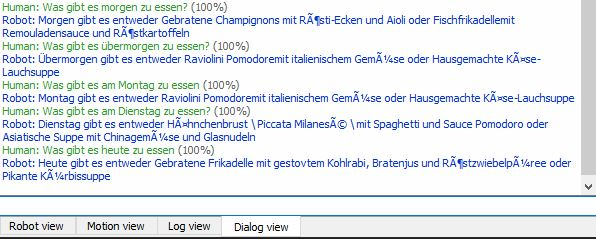
\includegraphics[width=\textwidth]{Figures/AppChapter/mensa_6.JPG}
    \caption{Mensa Dialog}
    \label{fig:mensadialog}
    \centering
\end{figure}


\section{Stundenplan}

Der zweite Anwendungsfall ist das Anzeigen des Stundenplans für jeden Studiengang und für jedes Semester. \\


\subsection{Anzeigen des Stundenplans in Android Studio}
Nachdem die Stundenplandaten im Server bereitgestellt wurden, war der nächste Schritt das Anzeigen des Stundenplans in Android Studio. 
Hierfür wurde ein neues Gesprächsthema in dem Haupt-Topic erstellt.\\

\begin{lstlisting}
u:({so} zeig{e} {er} {mir} {den} Stundenplan {fuer} {den} Studiengang 
_~Studiengaenge {[im "fuer das"]} semester _~semester {sofort} {bitte})

$course=$1 $semester=$2 Alles klar ^execute(VariableExecutor, 
timetable_course_semester, $course, $semester)
\end{lstlisting}

Damit der Anwender den Stundenplan einsehen kann, erwartet Pepper zwei Wörter. Der Anwender muss in seiner Frage den Studiengang und das Semester 
nennen. Erst dann wird der Methodenaufruf gestartet. Somit werden die drei Parameter \verb|timetable_course_semester|, 
\verb|course| und \verb|semester| mitgegeben.\\

\begin{lstlisting}[language=Java]
final String timetableurl = "https://informatik.hs-bremerhaven.de/
    docker-hbv-kms-http/api/v1/timetable?course="
    + course_ + "&semester="
    + semester_ + "&htmlOnly=true";

ma.runOnUiThread(() -> {
	ma.setContentView(R.layout.webtest);

	WebView web = (WebView) ma.findViewById(R.id.webView);
	WebSettings webSettings = web.getSettings();
	webSettings.setJavaScriptEnabled(true);
	web.setWebViewClient(new Callback());
	web.loadUrl(url);
});
\end{lstlisting}

Auf dem Node Server erwartet die API, die wir für den Stundenplan erstellt haben, bestimmte Parameter zu dem Studiengang und dem Semester. Hierfür können wir unsere Parameter, die in der Frage ermittelt wurden, in die Variable \verb|timetableurl| einsetzen und erhalten 
die URL zu dem richtigen Stundenplan. Dieser kann anschließend mit Hilfe des Webviewers auf dem Tablet von Pepper angezeigt werden. 

\section{Routenfinder}

Der dritte und letzte Anwendungsfall ist die Navigationshilfe in der Hochschule Bremerhaven. Sollte der Anwender einen bestimmten Raum oder ein Gebäude suchen, soll Pepper auf seinem Tablet eine genaue Wegbeschreibung geben können. 
\\
\textbf{Videos in /var/www/hbv-kms abgelegt}
\\


\subsection{Anzeigen des Gebäudeplans und des Raumfinders in Android Studio}

Da wir die einzelnen Videodateien auf dem Hopper abgelegt haben, brauchen wir für diesen Anwendungsfall die Kommunikation mit dem Node Server nicht. 
Die JSON Datei, die mit dem Python Script erzeugt wurde, haben wir in den /Assets Ordner in Android Studio abgelegt, um sie später im Code verwenden zu können. 

Wie bei allen anderen Anwendungsfällen auch, ist der erste Schritt das Erstellen der einzelnen Gesprächsthemen. 
Zuerst werden wir den Fall abdecken, wenn sich der Anwender den Gebäudeplan anzeigen lassen will.\\

\begin{lstlisting}
u:([zeig gib] {mir} {bitte} {den} [Gebaeudeplan Campusplan Gelaende])
^execute(VariableExecutor, qiVariableNav, Plan) Hier hast du eine 
    Uebersicht ueber das Hochschulgelaende
\end{lstlisting}


\begin{lstlisting}[language=Java]
String nav = params.get(1);
if(nav.equals("Plan")) {
    try {
        ma.runOnUiThread(() -> {
            ma.setContentView(R.layout.campus_plan);
        });
    } catch (Exception e) {
        e.printStackTrace();
    }
}
\end{lstlisting}

(vgl. Abb. \ref{fig:gplan}) Sobald der Anwender nach dem Gebäudeplan fragt, wird ein vordefiniertes XML-Layout mit einem Bild von dem 
Gebäudeplan auf dem Tablet angezeigt. Das Bild wurde vorher heruntergeladen und in den Ordner 
\verb|drawable| gelegt.\\

\begin{figure}[H]
    \centering
    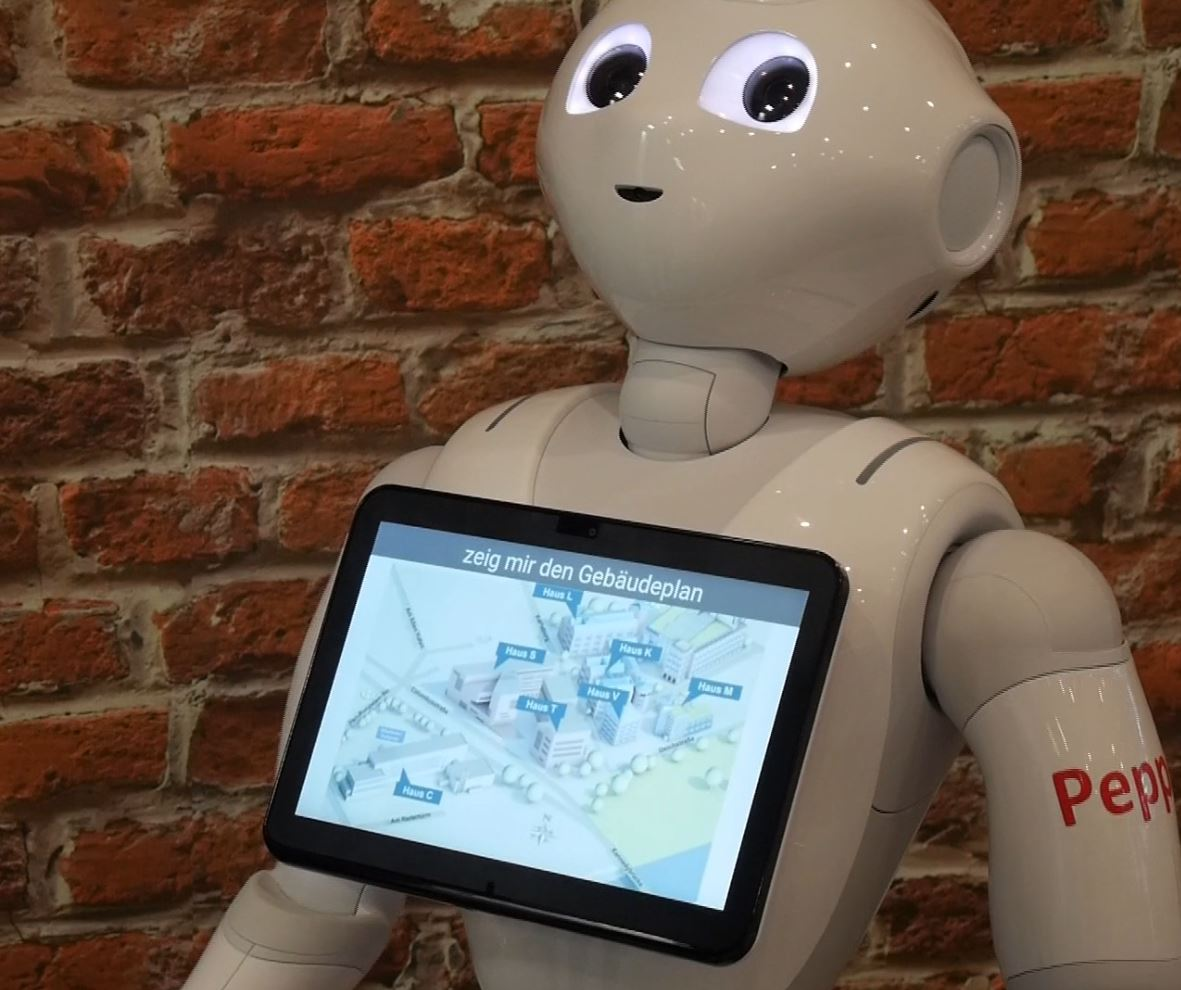
\includegraphics[width=10cm]{Figures/AppChapter/rx3.JPG}
    \caption{Gebäudeplan - Pepper}
    \label{fig:gplan}
    \centering
\end{figure}

Als Nächstes haben wir das Abrufen der Videodateien zu den einzelnen Räumen der Hochschule in Android Studio implementiert.\\

\begin{lstlisting}
concept:(rooms) [C006 C007 ... Z5150 Z5160 ]

u:(["{Kannst du {mir} [sagen erzaehlen]} Wo [befindet ist] {sich} der 
Raum _~rooms {befindet}"])
    $room=$1 Sofort ^execute(VariableExecutor, qiVariableNav, $room)
\end{lstlisting}

Pepper muss in der Lage sein, alle Räume in der Hochschule zu kennen, um genau herausfiltern zu können, welchen Raum der Anwender sucht. Das Concept \verb|rooms| beinhaltet alle Räume der Hochschule und wird somit in der Frage im Topic verwendet. Sollte der Anwender nach einen Raum fragen, den es nicht gibt, wird Pepper die Frage erst gar nicht verstehen und nicht antworten. 

Sollte Pepper den Raum kennen, wird ein Methodenaufruf mit den Parametern \verb|qiVariableNav| und der Raumnummer (\verb|room|) durchgeführt.\\

\begin{lstlisting}
u:(Zeig mir {bitte} einen _~handicapped Weg [zu in] {dem} 
Raum _~rooms)
    $handicap=$1 $room=$2 Alles klar ^execute(VariableExecutor, 
    qiVariableNav, $room, $handicap)
\end{lstlisting}

Wenn der Anwender explizit nach einem barrierefreien Weg zu einem Raum fragt, wird der gleiche Methodenaufruf mit dem zusätzlichen Parameter \verb|handicap| durchgeführt.\\

\begin{lstlisting}[language=Java]
String room = nav;
String handicapped = "M0000";
if(params.size() == 3) handicapped = "M0001";
\end{lstlisting}


In der \verb|VariableExecutor| Klasse wird als Erstes überprüft, ob der Anwender nach einem barrierefreien Weg zu dem gewünschten Raum gefragt hat oder nicht. Mit der If-Bedingung wird die Länge der Parameter überprüft, die in der Methode mitgegeben wurde. Wie bereits erwähnt, wird ein zusätzlicher Parameter \verb|handicap| zusammen mit den Parametern \verb|qiVariableNav| und \verb|room| mitgegeben, wenn nach dem barrierefreien Weg gefragt wurde. Somit muss nur die Parameterlänge verglichen werden, um entscheiden zu können, welcher Weg angezeigt werden soll.\\

\begin{lstlisting}[language=Java]
BufferedReader reader = new BufferedReader(new InputStreamReader(
    ma.getAssets().open("route_metadata.json")));

String response = new String();
for (String line; (line=reader.readLine())!=null; response+=line);

Map jsonJavaRootObject = new Gson().fromJson(response, Map.class);
String path = ((Map)((Map)(jsonJavaRootObject.get(room)))
    .get(handicapped)).get("video_path").toString();
\end{lstlisting}

Mit der \verb|getAssets().open("route_metadata.json")| Funktion, kann die JSON Datei, die sich in dem \verb|/assets| Ordner befindet, geöffnet und mit dem \verb|BufferedReader| ausgelesen werden. Als Nächstes wird mit Hilfe des \verb|Gson| Frameworks, ein Map Objekt erzeugt, dass alle Informationen der JSON Datei bereitstellt. In der Variable \verb|path|, wird der Wert 
\verb|video_path| mit Hilfe der genauen Raumnummer herausgefiltert. Hier wird auch die Abfrage mitgegeben, ob der Weg Barrierefrei sein soll oder nicht.\\


\begin{lstlisting}[language=Java]
String urlVideo ="https://informatik.hs-bremerhaven.de/hbv-kms/"+path;
try{
    ma.runOnUiThread(() -> {
        ma.setContentView(R.layout.webtest);
        WebView web = (WebView) ma.findViewById(R.id.webView);
        WebSettings webSettings = web.getSettings();
        webSettings.setJavaScriptEnabled(true);
        web.setWebViewClient(new Callback());
        web.loadUrl(urlVideo);
    });
}
\end{lstlisting}

(vgl. Abb. \ref{fig:Routenfinder}) Nachdem der genau Pfad zum Video ermittelt wurde, kann nun die URL zu dem Video erstellt und mit dem Webviewer angezeigt werden.\\

\begin{figure}[H]
    \centering
    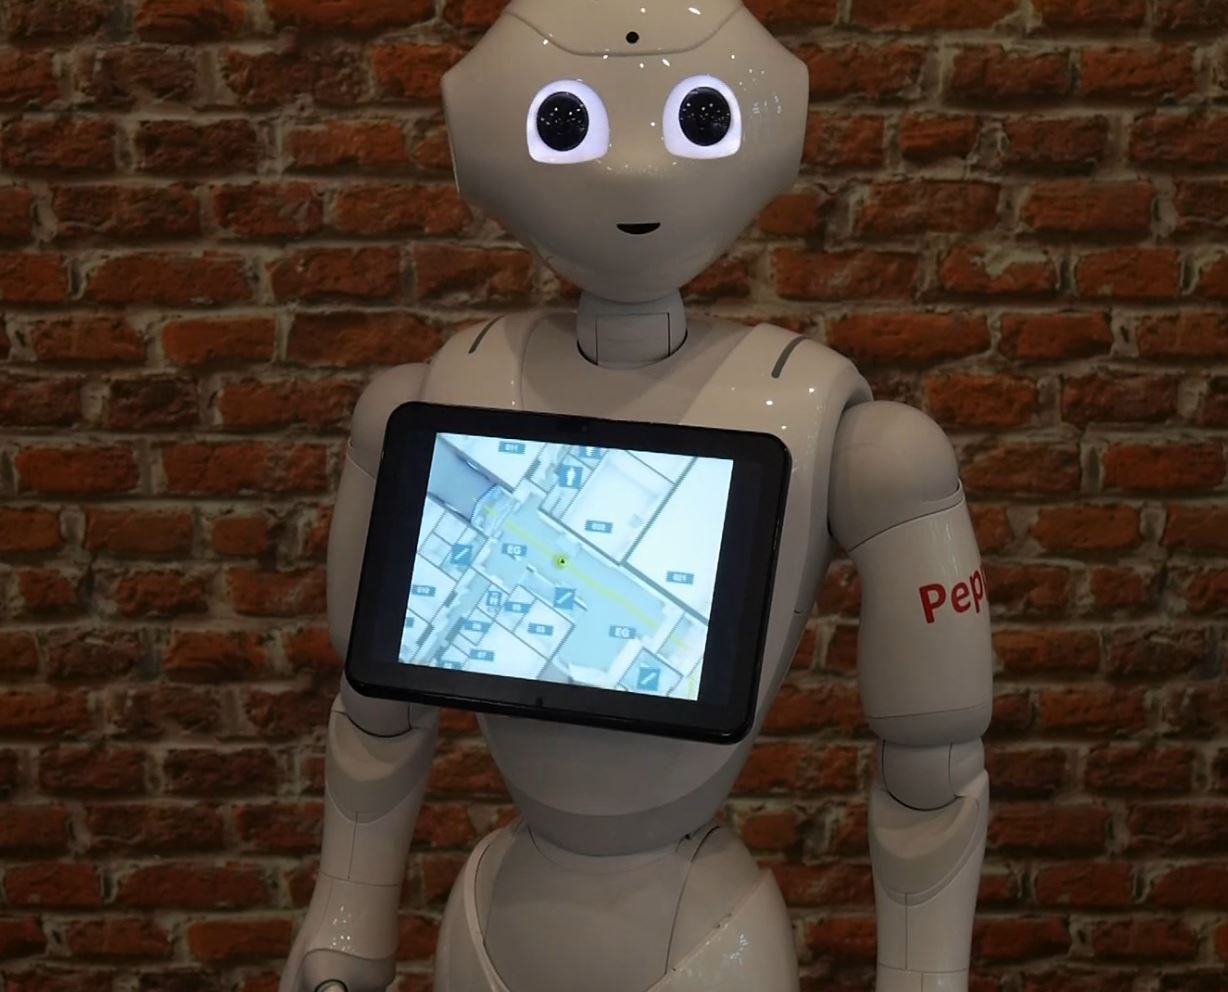
\includegraphics[width=10cm]{Figures/AppChapter/rx4.JPG}
    \caption{Routenfinder}
    \label{fig:Routenfinder}
    \centering
\end{figure}

(vgl. Abb. \ref{fig:RoutenfinderDia}) Zusätzlich zu dem Video soll Pepper dem Anwender mit zusätzlichen Details antworten. Er gibt an, in welchem Gebäude sich der gesuchte Raum befindet, 
wie weit dieser von seinem Standpunkt entfernt ist und wie viel Zeit benötigt wird, um diesen Raum zu erreichen.\\

\begin{figure}[H]
    \centering
    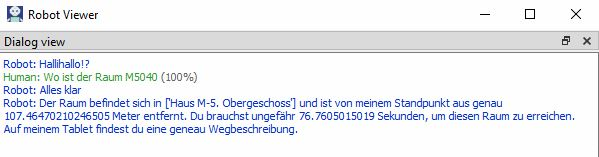
\includegraphics[width=\textwidth]{Figures/AppChapter/raumfinder_1.JPG}
    \caption{Routenfinder Dialog}
    \label{fig:RoutenfinderDia}
    \centering
\end{figure}

 % Implementierung: Anwendungsfälle 

\chapter{Skripte und Erweiterungen}
\label{sec:scripts}
\lhead{Kapitel 7. \emph{Skripte und Erweiterungen}}

 % Node - Express Server

\newcommand{\scripts}{Kapitel 8.}
\chapter{Skripte und Erweiterungen}
\label{chapter:scripts}
\lhead{\scripts \emph{Skripte und Erweiterungen}}

\section{Allgemein}
Neben der Anwendung für den Roboter Pepper und der Webanwendung haben wir weitere Skripte, hauptsächlich in Python, geschrieben. Diese sind in einem separaten Repository unter \href{https://github.com/ProjectPepperHSB/Backend-Services}{https://github.com/ProjectPepperHSB/Backend-Services} zu finden. In diesem Repositry befindet sich, wie in jedem anderen unserer Projekte auch, eine README.md, welche einen Einstieg in die Installation und Anwendung der einzelnen Skripte ermöglicht.

Es sind mehrere Verzeichnisse angelegt, welche separate Schwerpunkte beinhalten, auf welche wir in den folgenden Abschnitten genauer eingehen wedern. Auch diese bieten eigene README.md Dateien, welche die Installation, sowie deren Zweck aufzeigen.

In jedem dieser kleineren Module befindet sich eine \verb|install.sh|, sowie eine \verb|reguirements.txt| Datei, welche zusammen ausgeführt werden, um die für das Skript benötigten Packages zu installieren, sofern diese noch nicht vorhanden sind.

Es befindet sich auch ein Verzeichnis mit Namen \verb|analysis| in diesem Repository, jedoch gehen wir darauf im Kapiel \ref{chapter:big-data} genauer ein.\\

\section{Skripte zur Generierung von Dummy Konversationen}
\label{sec:dummy-data}
Aufgrund der andauernden Einschränkungen der Hygienemaßnahmen, ist es uns nicht möglich, Pepper an der Hochschule im vollem Umfang auszutesten. Somit können wir Pepper und seine Interaktionen nicht an einer großen Menge an Studierenden und Interessierten austesten. Da wir jedoch den Schwerpunkt Big Data mit in unserem Projekt einfließen lassen wollen und unsere Webanwendung, welche wir im Kapitel \ref{chapter:webapp} besprochen haben genau für das Sammeln und zur Verfügung stellen von Daten ausgelegt haben, war es für uns ganz klar, dass wir uns selbst Daten generieren müsssen.

Hierfür wurde ein Skript mit dem Namen \verb|create-dummy-data.py| geschrieben, welches über die Kommandozeile ausgeführt werden kann und mehrere Parameter übergeben bekommt.\\

\begin{lstlisting}[language=Bash]
    ~$ python3 create-dummy-data.py -n 1000 --prod
\end{lstlisting}

Das Flag \verb|n| gibt die Anzahl der zu generierenden Konversationen an. Das zweite Flag \verb|--prod| ist optioanl und sorgt dafür, dass die Daten, welche innerhalb des Skriptes generiert werden, an die URL der laufenden Webanwendung auf dem Hochschulserver gesendet werden. Ohne diesen Flag, werden die Datenreihen an den Localhost geschickt. Sollte dies nicht einwandfrei laufen, so ist die Webanwendung höchstwahrscheinlich nicht aktiv.

Da die \verb|requests| Library in Python nur synchrone Prozesse unterstützt und dies bei 1000 Anfragen etwas Zeit in Anspruch nimmt, haben wir dies mit der Library Joblib parallelisiert, sodass 6 Prozesse gleichzeitg die Generierung der Daten, sowie das Übermitteln an die Webanwendung übernehmen. Aufgurnd der Beschränkungen des Hochschulservers Hopper ist es nicht möglich, noch mehr gleichzeitige Anfragen zu schicken. Dies ist eine Sicherheitsmaßnahme zur Abwendung von DOS Attacken.\\


\section{Skripte für die Bereitstellung des Mensaplans}

Der Anwendungsfall für die Mensa ist in zwei Teile aufgeteilt. Der erste Teil ist das Anzeigen des Mensaplans auf dem Tablet von Pepper. Sollte der Anwender explizit nach dem Mensaplan fragen, muss Pepper in der Lage sein, eine Übersicht des Mensaplans der aktuellen Woche anzuzeigen. 
Der zweite Teil ist das verbale Beschreiben der Mensaangebote. Hierbei soll Pepper für jeden Wochentag erzählen können, welche Angebote in der Mensa zurzeit zur Verfügung stehen. Die Mensa der Hochschule Bremerhaven bietet jeden Wochentag immer zwei Angebote an. Das zweite Angebot ist dabei immer vegetarisch. Pepper muss dementsprechend in der Lage sein, beide Angebote beschreiben zu können. 

Um die verschiedenen Daten über die Mensa Angebote abrufen zu können, verwenden wir unseren Server, der diese Daten bereitstellt. Der Server bekommt diese Daten aus einem externen Python Script.\\

\subsection{Script um Mensadaten aufzurufen}
\label{sec:pyMensa}

Um die Daten auf dem Server anzeigen zu lassen, wird ein Python Script verwendet, dass sich diese Daten aus der offiziellen Hochschule Bremerhaven Mensa Webseite zieht. 

Webseite: \url{https://www.stw-bremen.de/de/cafeteria/bremerhaven}

Auf dieser Webseite befinden sich die aktuellen Angebote für die nächsten fünf Tage in einer Tabelle und den aktuellen- sowie nächsten Wochenplan im PDF-Format. Mit dem Script werden die einzelnen Daten aus der Webseite gelesen und als JSON gespeichert. Das Lesen der Daten aus der Webseite wird mit Hilfe des Frameworks \verb|BeautifulSoup| durchgeführt. Dieses Framework erlaubt es, XML- und HTML-Dokumente zu \verb|parsen|.\\

\begin{lstlisting}[language=Python]
menulist = soup.select('tbody')

menu, offer1, offer2 = {}, [], []
day: [str] = [
    'Montag', 'Dienstag', 'Mittwoch', 'Donnerstag', 'Freitag'
]
\end{lstlisting}

Die Mensa Angebote befinden sich auf der Webseite in einer Tabelle, weshalb wir auf alle \verb|tbody|-Elemente mit der Funktion \verb|soup.select| zugreifen. Diese werden als Array in die Variable \verb|menulist| initialisiert. Anschließend werden die Variablen deklariert, aus denen später der JSON string entstehen soll. \\

\begin{lstlisting}[language=Python]
for i in range(10):
    tmp = (str(menulist[i]).split('description">',1)[1]).rsplit
    ("</td><td",2)[0]
    tmp = tmp.replace('\n',').replace('\r',').replace('a1',')
    .replace('amp;',')
    tmp = re.sub('<sup>.*?</sup>', |, tmp)
    if(i%2==0): offer1.append(tmp)
    else: offer2.append(tmp)
    menu'"day'], menu['offer1'], menu['offer2'] = day, offer1, offer2

with open(folder_location+"mensadata.json", "w+") as f:
    json.dump(menu, f, ensure_ascii=False)
\end{lstlisting}

Da sich die Daten in den \verb|tbody|-Elementen schwer lesen lassen, werden diese mit mehreren \verb|split| und \verb|replace| Funktionen in lesbare Mensa Angebote umgeformt und in den einzelnen Variablen eingefügt. Die If-Bedingung wird verwendet, um das erste- und zweite Angebot voneinander zu trennen. Anschließend wird das \verb|menu| Objekt mit den keys \verb|day|, \verb|offer1| und \verb|offer2| und den Values der jeweiligen Arrays initialisiert.
Zum Schluss wird das \verb|menu| Objekt in JSON mit der \verb|json.dump| Funktion umgewandelt.

Um den aktuellen Wochenplan im Script herunterzuladen und weiterzuverarbeiten, wird die Programmbibliothek Poppler vorausgesetzt. Poppler wird in Unix-ähnlichen Betriebssystemen dazu verwendet, PDF-Dateien anzuzeigen.\\

\begin{lstlisting}[language=Python]
response = requests.get(url)
soup = BeautifulSoup(response.text, 'html.parser')
menucard = ((str(soup.select("a[href$='/print']")[0])
.rsplit(' target',1)[0]).split('href=',1)[1])
.replace('"',|)
urllib.request.urlretrieve(menucard, f'{folder_location}Mensaplan.pdf')
\end{lstlisting}

Mit den ersten beiden Zeilen des Codes wird der komplette HTML-Inhalt der Webseite in die Variable \verb|soup| initialisiert. Da wir die URL des aktuellen Wochenplans benötigen, muss dieser aus dem HTML Code gelesen werden. Der Standort dieser URL ist im HTML Code fest verankert, weshalb wir mit Hilfe von \verb|soup.select|, die URL herausfiltern und mit mehreren \verb|split| und \verb|replace| Funktionen zu einer gültigen URL umformen können. Dieser Zwischenschritt ist nötig, da sich die URL jede Woche ändert. Anschließend wird die URL aufgerufen und als \verb|Mensaplan.pdf| abgespeichert.\\

\begin{lstlisting}[language=Python]
img = convert_from_path(f'{folder_location}Mensaplan.pdf', 500)[0]

area = (0, 200, 4134, 2800) # R T L B
cropped_img = img.crop(area)

area = (0, 5200, 4134, 5800)
cropped_img2 = img.crop(area)
mergeImgs([cropped_img, cropped_img2])
.save(folder_location+'images/mensaplan.png', 'JPEG')
\end{lstlisting}

Im nächsten Schritt wird mit der Funktion \verb|convert_from_path| das PDF in ein Bildformat konvertiert und in die Variable \verb|img| installiert. Hierfür wird das Framework \verb|pdf2image| verwendet, das vorab mit \verb|pip| installiert werden muss. 

Nun ist das Bild jedoch im Hochformat und kann sehr schlecht auf dem Tablet von Pepper angezeigt werden. Somit haben wir das Bild in zwei Teile geschnitten und im Querformat zusammengefügt (vgl. Abb. \ref{fig:Mensaplan}). Um das Bild zu schneiden, haben wir das Framework \verb|PIL| verwendet. Nun kann genau angegeben werden, wie das Bild geschnitten werden soll. In der Variable \verb|area| haben wir jeweils immer vordefiniert, wie weit das Bild in welcher Richtung ausgeschnitten werden soll. Die Reihenfolge der Richtungen lautet wie folgt: 
(rechts oben links unten) (0, 200, 4134, 2800)

Zuerst haben wir den oberen Teil des Mensaplans ausgeschnitten, der die einzelnen Angebote enthält und anschließend die Legende, die sich im unteren Bereich der PDF befindet. 

Nun müssen beide Bilder zusammengefügt werden. Dies wurde in der Methode \verb|mergeImgs| durchgeführt.\\


\begin{lstlisting}[language=Python]
def mergeImgs(imgs):
    min_img_width = min(i.width for i in imgs)
    
    total_height = 0
    for i, img in enumerate(imgs):
    
    if(img.width > min_img_width):
        imgs[i] = img.resize((min_img_width, int(img.height / 
        img.width * min_img_width)), Image.ANTIALIAS)
    total_height += imgs[i].height
    
    img_merge = Image.new(imgs[0].mode, (min_img_width, total_height))
    y = 0
    for img in imgs:
        img_merge.paste(img, (0, y))
    
        y += img.height
    return img_merge
\end{lstlisting}

In dieser Funktion wird zuerst die Breite und Höhe des neu zusammengefügten Bildes ermittelt. Sollten die beiden Bilder eine unterschiedliche Breite besitzen, wird das breiteste Bild verkleinert. Dies geschieht in der For-Schleife, wo jedes einzelne Bild überprüft wird. 
Anschließend wir ein neues \verb|img_merge| Objekt erzeugt, das mit der minimalsten Breite und addierten Höhe der beiden Bilder initialisiert wird. Zum Schluss werden die beiden Bilder in das Objekt eingefügt und heruntergeladen.

\begin{figure}[H]
    \centering
    \includegraphics[width=15cm]{Figures/AppChapter/mensa_3.png}
    \caption{Mensaplan - cropped}
    \label{fig:Mensaplan}
    \centering
\end{figure}

\subsection{Weiterleitung zum NodeJS Server}

Das Script (vgl. Abschnitt \ref{sec:pyMensa}) befindet sich auf dem Hopper und wird mit \verb|crontab| jeden Montag einmal ausgeführt. Es ist wichtig, dass das Script nur jeden Montag ausgeführt wird, da die Mensa Angebote nur für die nächsten fünf Tage zur Verfügung kann. Sollte das Script zum Beispiel an einem Mittwoch ausgeführt werden, so würden die Tage Montag und Dienstag fehlen.\\

\begin{lstlisting}[language=Bash]
    # m h dom mon dow command
    0 0 * * 1 /usr/bin/python3 ~/getMensaPlan.py
\end{lstlisting}

Das erzeugte JSON Objekt und das zugeschnittene Bild des Mensaplans werden anschließend in den \verb|static| Ordner vom Node Server eingefügt.

\subsection{Bereitstellen der Mensadaten auf dem Server}

Mit dem folgenden Code werden die Daten aus den jeweiligen “/static” Ordnern an die Webseite gesendet:\\

\begin{lstlisting}[language=Java]
router.get('/docker-hbv-kms-http/api/v1/mensadata', (req, res) => {
    const filePath = `${__dirname}/../static/data/mensadata.json`;
    const jsonData = JSON.parse(fs.readFileSync(filePath, 'latin1'));
    res.send(jsonData);
});

router.get('/docker-hbv-kms-http/api/v1/mensadata/img', (req, res) => {
    const filePath = `${__dirname}/../static/images/mensaplan.png`;
    const img = fs.readFileSync(filePath);
    res.writeHead(200, {
        'Content-Type': 'image/png'
    });
    res.end(img, 'binary');
});    
\end{lstlisting}

(vgl. Abb. \ref{fig:mensaapi}) In folgendem Pfad befindet sich nun unser JSON Objekt, mit allen Mensaangeboten der aktuellen Woche.\\
\url{https://informatik.hs-bremerhaven.de/docker-hbv-kms-http/api/v1/mensadata}
\\
\begin{figure}[H]
    \centering
    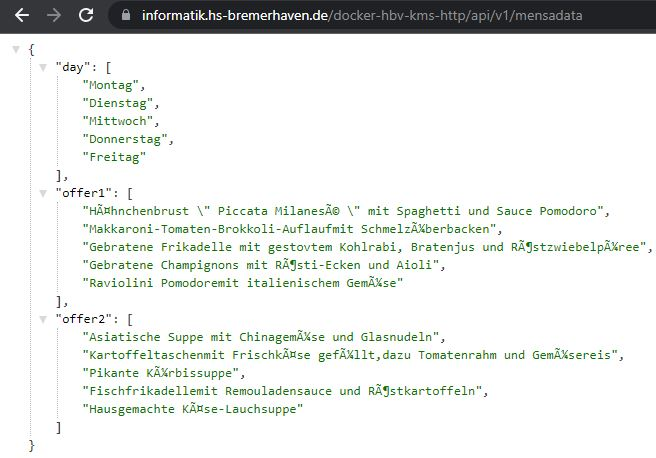
\includegraphics[width=13cm]{Figures/AppChapter/mensa_5.JPG}
    \caption{Mensadaten - API}
    \label{fig:mensaapi}
    \centering
\end{figure}

Der aktuelle Wochenplan ist in png-Format unter folgendem Link erreichbar:\\
\url{https://informatik.hs-bremerhaven.de/docker-hbv-kms-http/api/v1/mensadata/img}\\


\newpage
\section{Skripte für die Bereitstellung des 3D-Navigators}

Der Campus unserer Hochschule ist ziemlich weitläufig und unübersichtlich. Dazu kommt, dass mit der Zeit einige Gebäude von der Hochschule als Lernräume angemietet wurden, welche nicht direkt als solche zu erkennen sind. Aufgrund dessen erweist es sich, vor allem für Studenten der ersten Semester, sowie Besucher der Hochschule als äußerst schwierig, sich auf dem Campus zu orientieren.\\

\subsection{Anforderungen}
Die Benutzer des Roboters sollen die Möglichkeit haben, ihn nach einem Raum oder Ort zu fragen woraufhin Pepper eine genaue Wegbeschreibung als Antwort geben soll. Dabei ist es von Vorteil, dem Nutzer eine visuelle Beschreibung zu bieten, da die nicht nur einfacher zu verstehen ist, sondern auch mögliche Sprachbarrieren ausschließt. Dafür soll das Tablett von Pepper als visuelles Kommunikationsmittel für die Wegbeschreibung dienen. Über akustische Mitteilungen soll Pepper zudem eine geschätzte Dauer des Weges, sowie die Entfernung zu dem gesuchten Ort geben. Außerdem ist es wichtig, dass Pepper auch in der Lage ist, barrierefreie Wege für den Benutzer zu beschreiben, da unsere Hochschule auch barrierefreie Wege anbietet und körperlich beeinträchtigte Menschen nicht von einem solchen System nicht ausgeschlossen werden sollen.\\

\subsection{Vorhandene Ressourcen}
Bei der Suche im Web sind die ersten Ergebnisse für eine Orientierungshilfe oder einem Campusplan, die von der Hochschule Bremerhaven unter der offiziellen Internetseite der Hochschule Bremerhaven bereitgestellten Geländepläne. Diese bestehen aus einem 2-Dimensionalen Campusplan, wie in Abbildung \ref{fig:campus-integration} zu sehen, sowie einen 3-dimensionalen Campusplan (Abb. \ref{fig:campusplan}).\\

\begin{figure}[H]
    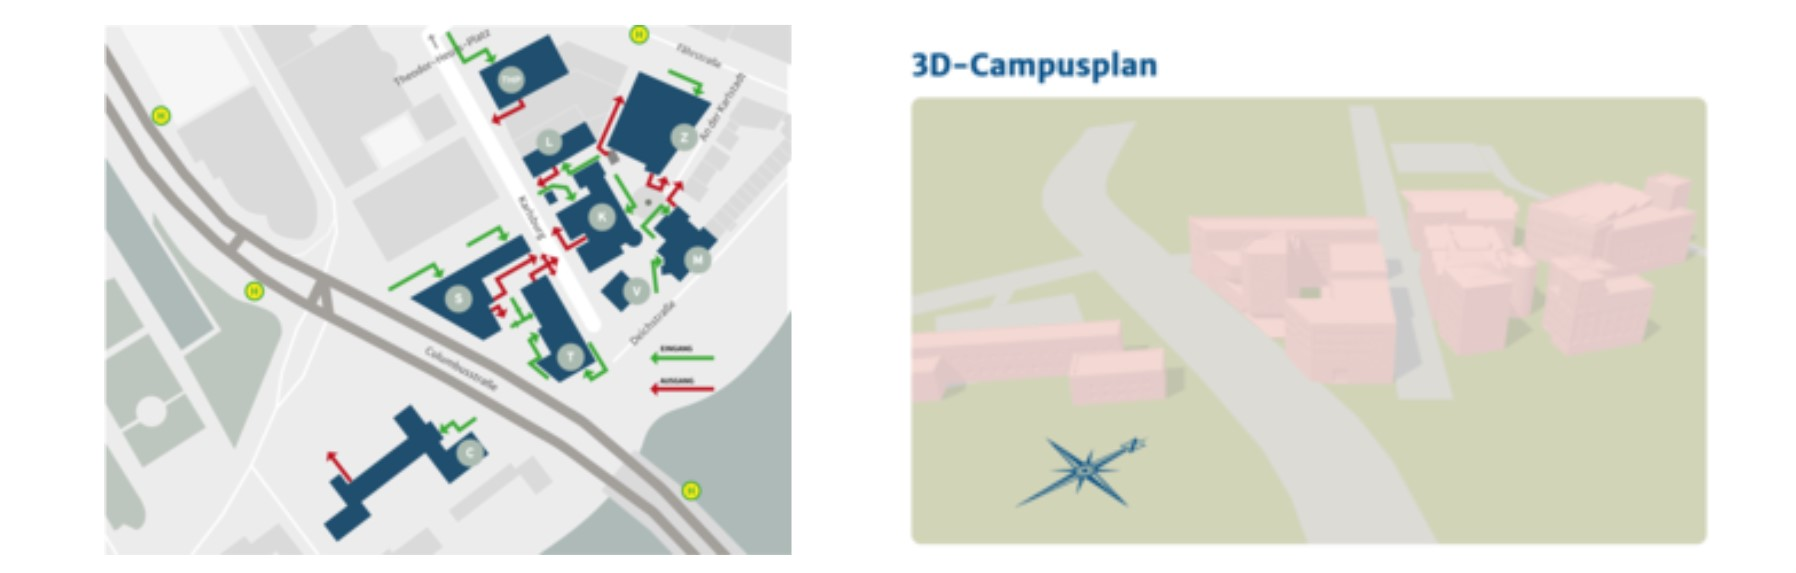
\includegraphics[width=\textwidth]{Figures/3DNavigator/campusplan_bsp.jpg}
    \caption{Beispiel: Zur Verfügung stehende Campuspläne}
    \label{fig:campus-integration}
    \centering
\end{figure}

Darüber hinsaus wird, auch vom AStA Bremerhaven, ein Campusplan bereitgestellt.\\

\begin{figure}[H]
    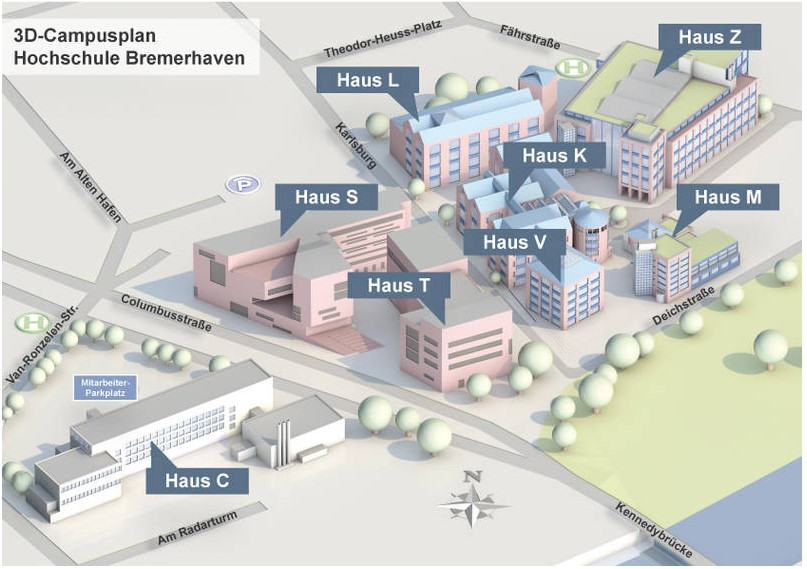
\includegraphics[width=\textwidth]{Figures/3DNavigator/asta_campusplan.jpg}
    \caption{Beispiel: AStA Campusplan}
    \label{fig:campusplan}
    \centering
\end{figure}

Alle diese Karten haben gemeinsam, dass sie einem zwar einen Überblick über das Campusgelände bieten, wodurch eine, nach einem bestimmten Raum suchende, Person zwar in der Lage wäre, das passende Haus zu finden, allerdings ist es dort angekommen, immer noch notwendig, den richtigen Raum, mit der entsprechenden Nummer zu finden. Ein weiteres Problem dieser Gebäudepläne ist auch, dass es zwar anhand des Buchstaben vor der zu suchenden Raumnummer möglich ist, das richtige Gebäude zu finden, jedoch nicht, das Haus zu finden, in dem sich beispielsweise die Mensa oder die Bücherei befindet. Da wir vorhaben, Pepper den Weg zu einem bestimmten Ort oder Raum genau beschreiben zu lassen, wäre es mit einem solchen Campusplan ein ziemlich großer Aufwand visuelle Markierungen, in Form von Linien, in die Pläne abbilden zu lassen. Außerdem gibt damit immer noch das Problem, die genaue Route innerhalb eines Gebäudes zu bestimmen, vor allem dann, wenn barrierefreie Wege gewünscht sind. Zudem müssten wir die sprachlich ausgegebenen Informationen zu den Wegrouten selbst erzeugen, was einen sehr großen Aufwand darstellen würde.

Aufgrund dieser genannten Gründe, eignet sich also ein solcher Gebäudeplan relativ schlecht für unser Vorhaben, Pepper sinnvoll und effizient für die 3D-Navigation auf dem Campusgelände zu nutzen. Wir haben uns deswegen für eine, von 3D-Berlin, zur Verfügung gestelltes, schlüsselfreies API-System entschieden. Diese API wurde von Prof. Dr.-Ing. Peter Ritzenhoff 2014 im Auftrag der Hochschule Bremerhaven von der 3D-Derlin VR Solutions GmbH erstellt. Sie besteht aus einem in 3-dimensional, visualisierten Modell der Hochschule Bremerhaven, in welchem die Räume anhand der Gebäudepläne Maßgetreu animiert wurden.\\

\begin{figure}[H]
    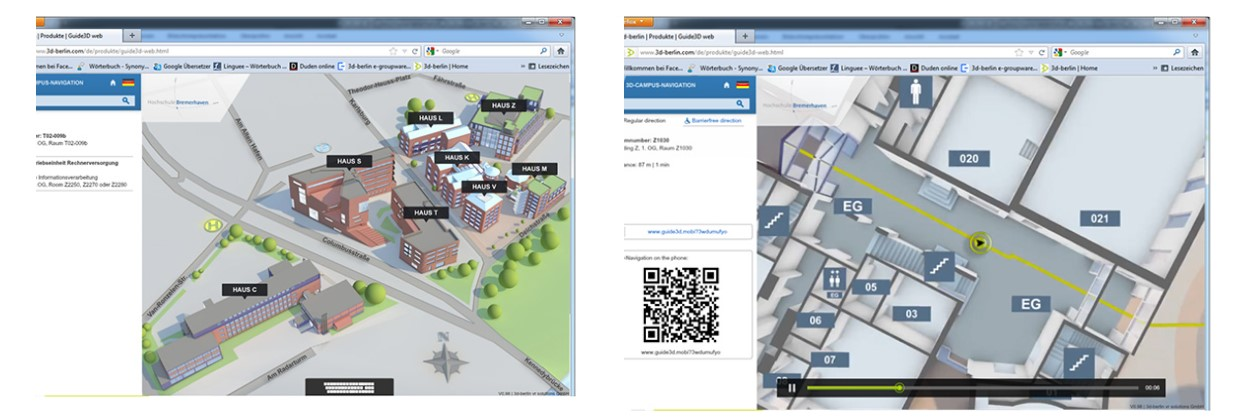
\includegraphics[width=\textwidth]{Figures/3DNavigator/3d-berlin_bsp.jpg}
    \caption{Beispiel: 3D-Berlin, 3D Navigator API}
    \label{fig:3dberlin-images}
    \centering
\end{figure}

Dieses API-System wurde genau für solch einen Anwendungsfall, wie wir ihn erstellen wollen, entwickelt. Für gewöhnlich werden diese wie von 3d-Berlin entwickelten 3D-Navigation in großen Gebäudekomplexen und Kaufhäusern verwendet, um sie dann auf digitalen Endgeräten wie Smartphones oder Digitalterminals für Besucher zur Orientierung zu Verfügung zustellen (Abb. \ref{fig:kaufhausbilder}).\\

\begin{figure}[H]
    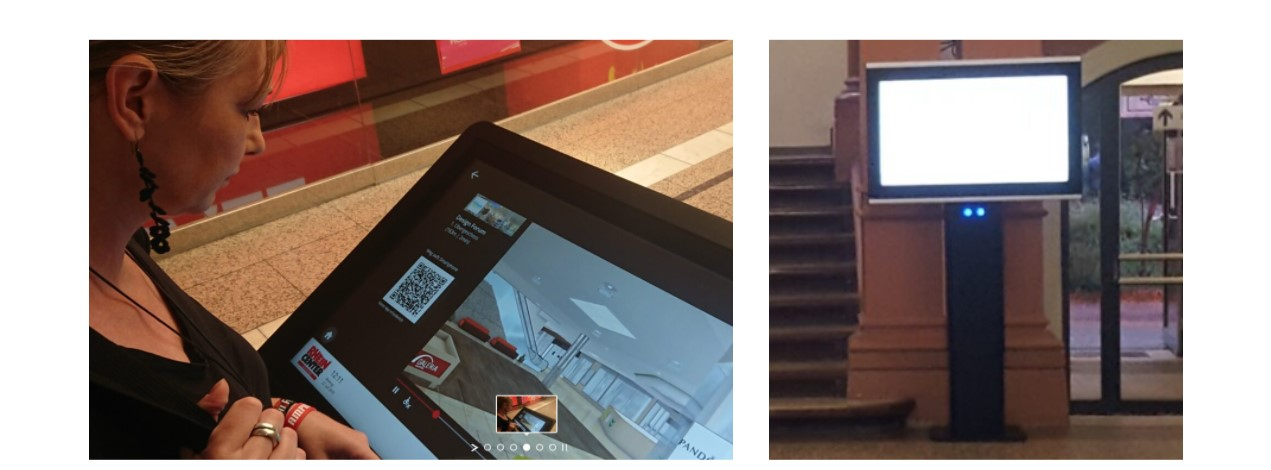
\includegraphics[width=\textwidth]{Figures/3DNavigator/terminal_bsp.jpg}
    \caption{Beispiel: Terminal für Kaufhäuser}
    \label{fig:kaufhausbilder}
    \centering
\end{figure}

Die Implementierung eines solchen 3D-Navigators stellt also eine innovative Anwendung dar. Wir verfügen mit dieser API über die Möglichkeit, einen Start- und Endpunkt als Anfrage an die API zu schicken und daraufhin per HTTP ein passendes Video, mit dem genauen Ablauf der Route als Antwort zu bekommen. Ein weiterer Vorteil ist, dass die wir die Distanz in Meter, sowie die geschätzte Dauer für eine Route zwischen zwei Räumen abfragen können, wodurch wir diese Informationen von pepper verbal ausgeben zur Verfügung stellen können, während das Tablet ein Video für die Wegbeschreibung abspielt. Anschließend zeigt jedes von dieser API ausgelieferte Video, einen QR-Code mit einem Link zu dem entsprechenden Video. Dieser QR-Code lässt sich von einem Benutzer mithilfe eines Smartphones einscannen, wodurch sich die Route auch nach Antreten des Weges problemlos nachvollziehen lässt. Außerdem ist die API in der Lage, ein Video mit der Wegbeschreibung für einen barrierefreien Weg zu erstellen, womit die Nützlichkeit des 3D-Navigators noch mehr Anwendungsbereiche abdeckt.\\

\subsection{Entwicklung und Implementierung des 3D-Navigators}

Wir haben uns dazu entschieden, die Daten des 3D-Navigators auf dem Hochschulserver Hopper bereitzustellen. Dies bietet den Vorteil, dass wir unabhängig von der Verfügbarkeit der 3D-Berlin API sind. Zudem sind wir so in der Lage, die Struktur der benötigten Daten selbst zu definieren, um sie möglichst effizient von Pepper abrufen zu lassen. Zunächst haben wir das Vorgehen für die Erstellung des Navigators geplant, wobei wir es für sinnvoll erachten, das Vorgehen in 5 verschiedene Schritte aufzuteilen. Die Abbildung zeigt die chronologische Vorgehensweise bei der Entwicklung, sowie die primär verwendete Programmiersprache, so wie weitere benötigte Technologien, um das Ziel des jeweiligen Schrittes zu erreichen.\\

\begin{figure}[H]
    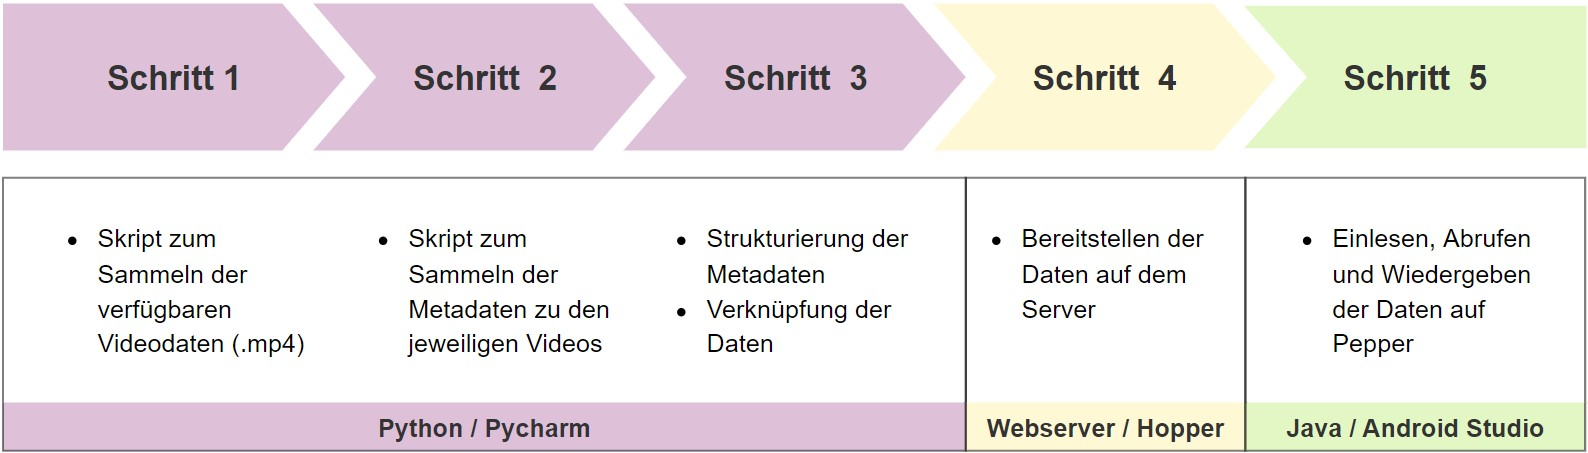
\includegraphics[width=\textwidth]{Figures/3DNavigator/Implementierungdes3DNavigators.jpg}
    \caption{Vorgehen: Entwicklung des 3D-Navigators}
    \label{fig:dev-navigator}
    \centering
\end{figure}

\subsubsection{Planung der Videodaten-Struktur}

Die Strukturierung der Videos soll so erfolgen, dass es bei der fertigen Implementierung für die Kommunikation zwischen Pepper und dem Server möglichst unproblematisch, sowie effizient ist, das passende Video zu der benötigten Anfrage abzurufen. Außerdem ist es aufgrund der speziellen Sonderzeichen innerhalb einiger Raumnamen nicht möglich, die Namen der Räume direkt innerhalb der Deklaration der Videodateien zu verwenden. Die Struktur der Dateinamen besteht deswegen aus drei notwendigen Informationen, diese sind dabei der Übersicht halber mit einem ``-'' Zeichen voneinander getrennt und bilden immer einen, nur einmalig vorkommenden, Namen zur Wiedererkennung des jeweiligen Videos. In der ersten Sektion befindet sich die ID für den Startpunkt der Route und in der zweiten die des zu erreichenden Endpunktes. Die Definition dieser Identifikationsnummern sind dieselben ID-Namen, wie sie die API von 3D-Berlin verwendet hat. Das hat den Vorteil, dass wir im Nachhinein besser nachvollziehen können, aus welcher Anfrage das entsprechende Video ursprünglich stammt. Zudem wäre es ineffizient, eine neue Nummerierung der ID's anzulegen. Der dritte Abschnitt des Videonamens beschreibt, ob es sich um ein Video mit einem Barrierefreien Weg oder um einen gewöhnlichen Weg handelt. Dabei steht die Bezeichnung ``M0000'' für den gewöhnlichen Weg und ``M0001'' für einen Weg unter Berücksichtigung der Barrierefreiheit. Somit gibt es für jedes Video also zwei verschiedene Varianten. Die untere Abbildung soll eine Abstrahierung dieser Datenstruktur verdeutlichen.\\

\begin{figure}[H]
    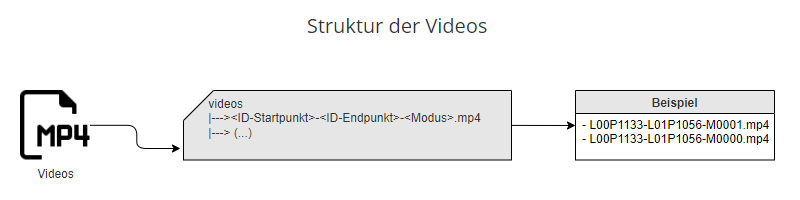
\includegraphics[width=\textwidth]{Figures/3DNavigator/Videostruktur_Raumfinder.png}
    \caption{Datenstruktur: Wegrouten Videos}
    \label{fig:raumfinder-videostruktur}
    \centering
\end{figure}\vspace{-2.5mm}

Bei dem Format der Videos haben wir uns für \verb|mp4| entschieden. Diese Videodateien verfügen über eine gute Browserkompatibilität und bieten trotz einer verhältnismäßig geringen Speichergröße trotzdem eine möglichst hohe Bildqualität. Da wir bei jeder Anfrage einer Wegbeschreibung das entsprechende Video per HTTP vom Server an den Roboter senden, eignet sich dieses Format also gut, da wir so eine entsprechend geringe Verzögerung beim Übertragen und Anzeigen des Videos erreichen. Wir haben uns deswegen auch für eine Bildbreite von 306px und eine Bildhöhe von 544px entschieden, wodurch wir eine durchschnittliche Größe von 1.5MB pro mp4-Datei kommen. Insgesamt soll Pepper in der Lage sein ca. 500 verschiedene Wegbeschreibung zu abzubilden, wodurch sich ein Datensatz von ca. 1.000 mp4-Videos mit insgesamt 845MB Kapazität ergibt.\\

\subsubsection{Sammeln der Videodaten}

Zunächst haben wir uns einen Überblick darüber verschafft, welche Daten wir mithilfe der 3D-Berlin API erhalten können. Als geeignetes Werkzeug für das automatisierte Arbeiten mit Requests haben wir uns für die Programmiersprache Python entschieden. Python bietet uns die Möglichkeit, schnell und zielorientiert, ein effizientes Skript zu entwickeln, um die benötigten Daten nicht nur auszulesen, sondern auch zu formatieren und sie später direkt in unsere gewünschte Datenstruktur einzubinden. Das Pythonskript \verb|createvideodata.py| ist Teil unserer Backend Anwendungen und dient dazu, die erforderlichen Anfragen für den Download der Videos zu konstruieren. Anschließend werden diese ausgeführt und mit dem richtigen Dateinamen zu versehen. Ein paar relevante Ausschnitte des Skripts möchten wir im Folgenden erläutern.
Um genau zu wissen, welche Wegrouten wir erzeugen können, rufen wir zunächst eine Liste der Video-IDs ab. Wir bekommen diese in Form einer JSON-Datei als Antwort zurück und initialisieren die Variable ``videos'' mit ihr.
Ist ein Request erfolgreich ausgeführt wurden, so speichern wir die erhaltene MP4-Datei zwischen und schreiben sie in das vorab gewählte Verzeichnis für die Videos.\\
\begin{lstlisting}[language=Python, caption={speichern der Videodaten}]
    open(f'{directory}/{video_name}', 'wb').write(response_object.content)
\end{lstlisting}
% \begin{figure}[H]
%     
\includegraphics[width=\textwidth]{../Figures/3DNavigator/code04.jpg}
%     \centering
% \end{figure}\vspace{-4.5mm}

Als letztes haben wir das Skript mit Hilfe des ``PySimpleGUI''  Frameworks noch um eine Grafische Oberfläche erweitert. Mit diese sind wir in der Lage, nachhaltig das Verzeichnis zum Speichern der Videos über den windows-explorer auszuwählen. Zudem haben wir einen Ladebalken implementiert, welcher den Fortschritt des Downloads anzeigt. Abbildung \ref{fig:gui-route} zeigt die von uns erstellte grafische Anwendung und den Output des Skripts:

\begin{figure}[H]
    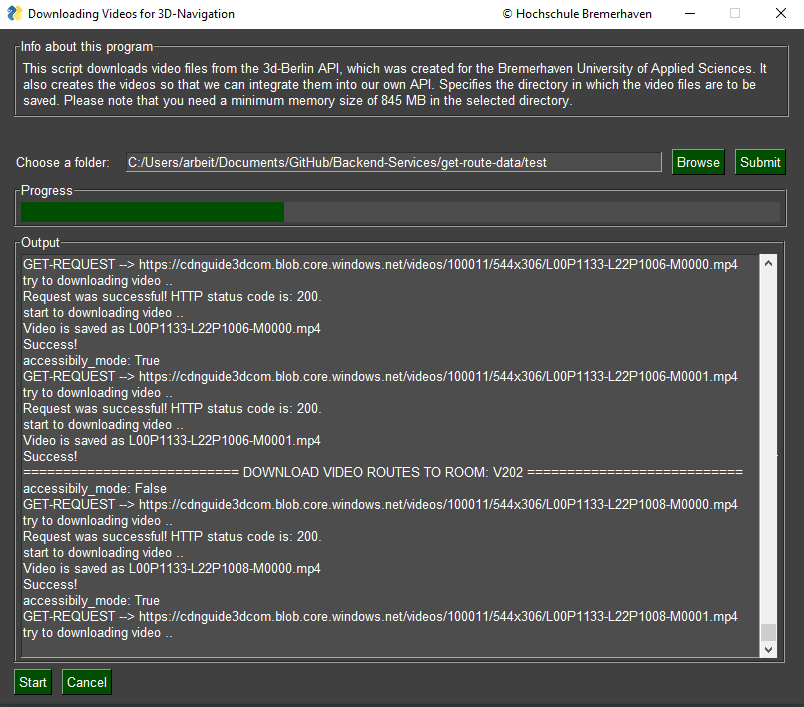
\includegraphics[width=\textwidth]{Figures/3DNavigator/create_videodata_pic.png}
    \caption{Screenshot: Grafische Oberfläche des Download-Skripts}
    \label{fig:gui-route}
    \centering
\end{figure}\vspace{-2.5mm}

Ist das Skript durchgelaufen haben wir die Videos erfolgreich in die geplante Struktur und mit der korrekten Deklaration der Dateinamen in ein Verzeichnis gespeichert.\\

\subsubsection{Planung der Datenstruktur für die Routeninformationen}

Die Strukturierung der Metainformationen soll so gestaltet werden, dass es für Pepper und den Server möglichst einfach ist, das passende Video zu der erfolgten Anfrage abzurufen. Die Metainformationen über die Wegbeschreibungen zu einem Raum setzen sich aus folgenden Attributen zusammen:\vspace{5mm}

\begin{tabular}{| l | p{9.45cm} | c| } \hline
    \multicolumn{3}{|c|}{\textbf{Attribute einer Wegroute}}                                                                                                                                                                                                                                                                                                                                                                                                                                                                                                                                                                                                                                                                                                                                                                                                                         \\ \hline\hline
    Beschreibung                                                                                                                                                                                                                                                                                                                                                                                                                                                                                                                                                    & Kommentar                                                                                                                                                                                                                                                                                          & Datentyp \\
    \hline
    Art des Weges                                                                                                                                                                                                                                                                                                                                                                                                                                                                                                                                                   & \small Es gibt zu jeder Wegbeschreibung zwei verschiedene Arten, das Ziel
    zu erreichen. Dabei bilden wir jeweils einen barrierefreien und einen gewöhnlichen
    bzw. schnell zu erreichenden Weg an. Obwohl es nur zwei verschiedene Zustände für die Art eines Videos gibt, haben uns hierbei bewusst für einen String und nicht für einen booleschen Wert entschieden. Der Grund dafür ist, dass sich bei der Erstellung des Skriptes () gezeigt hat, dass wir so keine Datentypen bei der Strukturierung eines Requests umwandeln müssen. Außerdem haben wir so die Möglichkeit über genügend Agilität zu verfügen, sollten wir dieses Skript zukünftig für ein Projekt werden wollen, welches mehr als zwei Modi verwendet. & String                                                                                                                                                                                                                                                                                                        \\[0.5ex]
    \hline
    Videopfad                                                                                                                                                                                                                                                                                                                                                                                                                                                                                                                                                       & \small Dieser Parameter stellt die direkte Verknüpfung zu der entsprechenden Daten mit der dazugehörigen Rauminformation dar. So können wir möglichst präzise das passende Video mit der richtigen Wegbeschreibung ermitteln.
                                                                                                                                                                                                                                                                                                                                                                                                                                                                                                                                                                    & String                                                                                                                                                                                                                                                                                                        \\
    \hline
    Ort                                                                                                                                                                                                                                                                                                                                                                                                                                                                                                                                                             & \small Der Ort ist eine kurze Beschreibung, in welchem Haus und welcher Etage sich der Raum befindet. Eine solche Ortsbeschreibung wäre zum Beispiel “Haus C Erdgeschoss”. Mit dieser Umschreibung kann Pepper dem Benutzer noch eine zusätzliche Information für eine verbale Interaktion bieten. & String   \\
    \hline
    Distanz                                                                                                                                                                                                                                                                                                                                                                                                                                                                                                                                                         & \small Bei der Distanz geben wir die Entfernung, ausgehend vom Startpunkt der Wegbeschreibung bis zum Ziel an. Wir verwenden dabei Meter als Einheit und runden diese für eine bessere Verständlichkeit auf ganze Meter auf.                                                                       & Integer  \\
    \hline
    Dauer                                                                                                                                                                                                                                                                                                                                                                                                                                                                                                                                                           & \small Die Dauer geben wir in Minuten an. Sie beschreibt die benötigte Zeit vom Startpunkt bis zum Ziel, ausgehend von der durchschnittlichen Schrittgeschwindigkeit.                                                                                                                              & Integer  \\
    \hline
\end{tabular} \vspace{5mm}

Anschließend haben wir begonnen, die zur Verfügung stehenden Eigenschaften der Wegrouten sinnvoll miteinander zu verknüpfen.% und in Relation untereinander zu betrachten. 
Dabei sei vorausgesetzt, dass die Informationen immer zu genau einem Video gehören und dabei möglichst einfach zu finden sein sollen. Außerdem gibt es zu jedem Raum, genau zwei verschiedene Wegbeschreibungen, da wir zwischen dem normalen und dem barrierefreien Weg unterscheiden müssen. Dies hat zur Folge, dass zu jeder Wegroute, zwei verschiedene Eigenschaften zur Verfügung stehen müssen, welche sich jedoch die gleiche Art und Struktur der Datentypen teilen. Diese Beziehungen der Daten zueinander haben wir der Übersicht halber in einem Entity-Relationship-Modell charakterisiert.

\begin{figure}[H]
    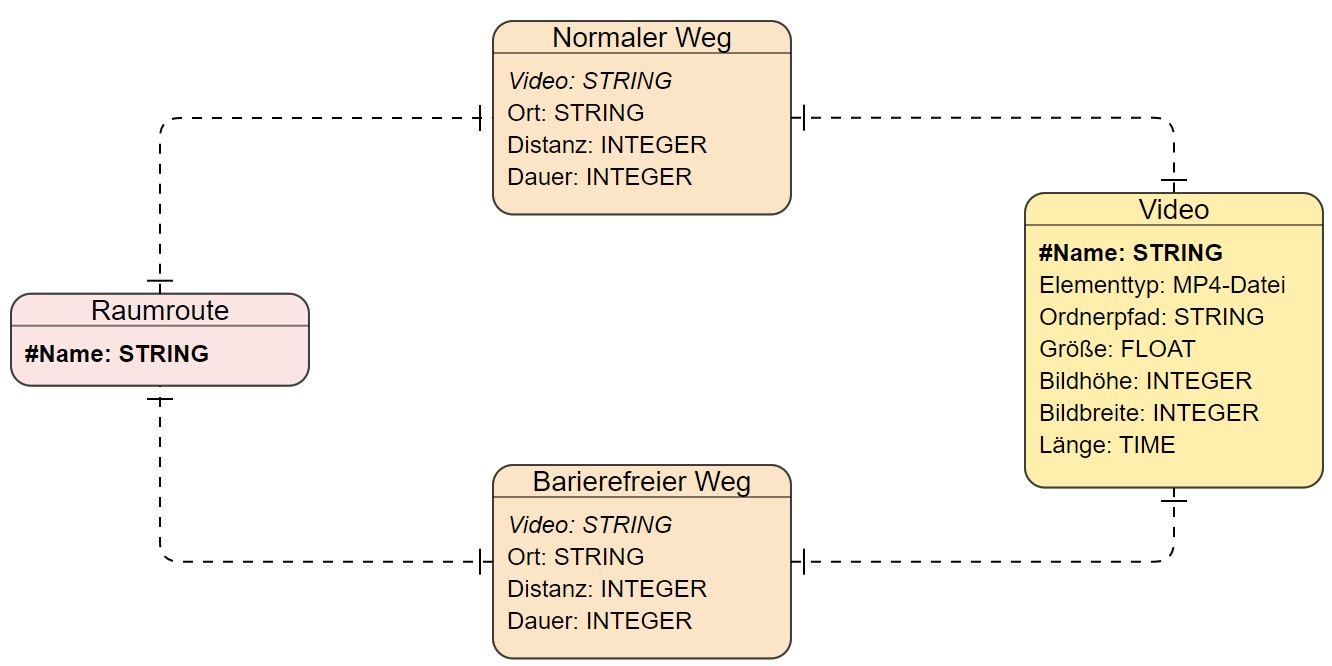
\includegraphics[width=\textwidth]{Figures/3DNavigator/EntityrelationshipdiagrammRaumfinder.jpg}
    \caption{Diagramm: ER-Modell der Wegrouten Informationen}
    \label{fig:integration}
    \centering
\end{figure}

Mit Hilfe dieses Datenmodells, konnten wir ein passendes Datenformat für unseren Anwendungsfall wählen. Wir haben uns dabei für die JavaScript Object Notation entschieden, da dies uns den Vorteil bietet, Datenstrukturen in lesbarer Form abzubilden. Außerdem verfügen wir so über ein Datenformat, welches eine hohe Unabhängigkeit von Programmiersprachen bietet. Dies erweist sich für unsere Architektur als äußerst vorteilhaft, da wir zwischen unseren Anwendungen und Entwicklungsabläufen verschiedene Programmiersprachen verwenden. Die endgültig geplante Struktur der JSON-Datei haben wir unten in der Abbildung \ref{fig:json-bild} abstrahiert dargestellt.

\begin{figure}[H]
    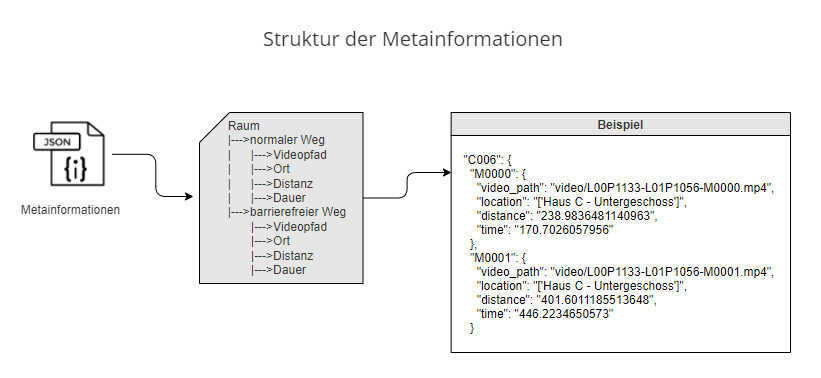
\includegraphics[width=\textwidth]{Figures/3DNavigator/Metadatenstruktur_Raumfinder.png}
    \caption{Datenstruktur: Abstrahierung der Wegrouten Informationen}
    \label{fig:json-bild}
    \centering
\end{figure}

\subsubsection{Sammeln der Wegroutendaten}
\label{sec:jsonget}
In der Dokumentation von 3D-Berlin wird ausschließlich beschrieben, wie die entsprechenden Anfragen für die geforderten Videos zu definieren sind. Aus diesem Grund sind wir so vorgegangen, dass wir mithilfe des Netzwerkanalysetools unseres Browsers die Antworten der gesendeten Anfragen, während der Nutzung des 3D-Navigators beobachtet haben. Dabei konnten wir genau ermitteln, welche Anfragen notwendig sind, um weitere Daten über die Videos zu erhalten und wie diese in ihrer Struktur aufgebaut werden müssen.

Auch hier haben wir uns für die Programmiersprache Python entschieden. Dafür haben wir innerhalb unseres Backends ein weiteres Skript, \verb|createmetadata.py|,angelegt. Das Skript beschafft sich die Informationen, welche wir unter der API 3D-Berlin finden konnten und wandelt diese in für uns brauchbare Daten um. Außerdem werden diese anschließend in der Datei \verb|routedata.json| gespeichert. Im Folgenden gehen wir auf ein paar relevante Abschnitte des Skripts genauer ein und erläutern diese.

Zu Beginn werden zwei verschiedene Requests definiert. Der Erste erzeugt das Request-Objekt für den normalen Weg und der Zweite generiert das gleiche Request-Objekt als barrierefreie Route.

\begin{lstlisting}[language=Python, caption={definieren der Anfragen}]
        r_M0 = get_request(mode='M0000',
                           project=project,
                           startpoint=startpoint,
                           endpoint=endpoint)
        r_M1 = get_request(mode='M0001', 
                           project=project, 
                           startpoint=startpoint, 
                           endpoint=endpoint)

\end{lstlisting}

Die Funktion “getrequest()” bekommt als Übergabeparameter einen String “mode” übergeben. Dieser Parameter gibt an, um welche Variante der Route es sich handelt. Außerdem wird eine Projekt-ID “project” übergeben. Über diese ID lässt sich das von uns an die API angeforderte Projekt bestimmt. Wir haben diesen Parameter bewusst variabel implementiert, um das gesamte Skript flexibel für einen möglichen weiteren Anwendungsfall im Zusammenhang mit 3D-Navigations APIs von 3d-Berlin zu gestalten. Es werden zudem ein Start “startpoint” sowie ein Endpunkt ``endpoint'' an die Funktion übergeben. Diese geben an, von welchem Startpunkt aus, welches Ziel zu erreichen sein soll. Es sei dazu gesagt, dass bei jeder Route immer von demselben Startpunkt ausgehen. Dies hat einerseits den Grund, dass der notwendige Datensatz an MP4-Dateien sonst exponentiell steigen würde und wir somit nicht in der Lage während diese Speicherkapazität auf dem Hopper-Server zu gewährleisten. Ebenso setzen wir für unseren Anwendungsfall des Roboters als Hochschulassistenz voraus, dass dieser sich immer an dem gleichen Ort befindet. Es handelt sich bei dem Startpunkt um das Foyer in Haus K. Wir haben auch diesen Parameter dennoch variabel gelassen, um unsere Anwendung so flexibel wie möglich zu entwickeln.\\

\begin{lstlisting}[language=Python, caption={Aufbau der Request-Funktion}]
    def get_request(mode, project, start_point, end_point):
        return requests.get(
            url=f'https://services.guid3d.com/route/cors/index.php?\
            project={project}&start={start_point}&end={end_point}\
            &mode={mode}&redirect=duration&format=none',
            allow_redirects=True
        )
\end{lstlisting}

Als Nächstes wird über die Liste der Videos iteriert, um den Request für die Anfrage der Routeninformation für genau jedes Video zu erstellen.
Innerhalb dieser Schleife lesen wir als Erstes den Raumnamen und aus der Beschreibung des Ortes ungewollte Zeichen aus dem String heraus. Dies ist notwendig, da es sonst später in der Android-Applikation erfolgen müsste und eine überflüssige Prozessbelastung darstellen würde. Danach werden die Gleitkommazahlen der Dauer und der Distanz einer Route auf ganze Zahlen, als Integer aufgerundet. Außerdem werden die Sekunden in Minuten umgerechnet.

\begin{lstlisting}[language=Python, caption={erstellen der JSON-Datei mit den Wegrouteninformationen}]
    new_json_struct.update(
        {
            f'{room_name}: {
                'M0000':{
                    'path': f'{v_path}M0000.mp4',
                    'location': location,
                    'distance': distance_M0,
                    'time': duration_M0,
                },
                'M0001':{
                    ...
                },
                {...}
            }
        }
    )
\end{lstlisting}


Es wird nun ein temporäres JSON-Objekt für die jeweilige Wegroute erzeugt. In dieser wenden wir die zuvor geplante Struktur der Informationen an und weisen die Values den entsprechenden Key zu. Danach wird jedes Objekt an die endgültige JSON-Datei angeknüpft.

Wir haben auch für diese Anwendung nachträglich eine grafische Oberfläche implementiert, um das Ausführen des Programms übersichtlicher und nachhaltiger zu gestalten. Dabei haben wir die Oberfläche so gestaltet, dass wir zwei verschiedene Konsolen für die Outputs anzeigen lassen. Die Linke Ausgabe ist die des Programmablaufs. Auf der rechten Ausgabe sind die hinzugefügten JSON-Objekte aufgelistet. In der folgenden Abbildung ist ein Durchlauf des Programms zu sehen. Es gibt die Möglichkeit ein Zielverzeichnis und den namen für die zu erstellende Datei zu wählen. Werden diese beiden Eigenschaften nicht zuvor gesetzt und mit einem Klick auf die ``Submit'' Schaltfläche bestätigt, so bekommt die Datei den namen ``routedata'' und wird in das Verzeichnis \verb|video| geschrieben. Die Abbildung unten zeigt das laufendene Programm:\vspace{-1.5mm}

\begin{figure}[H]
    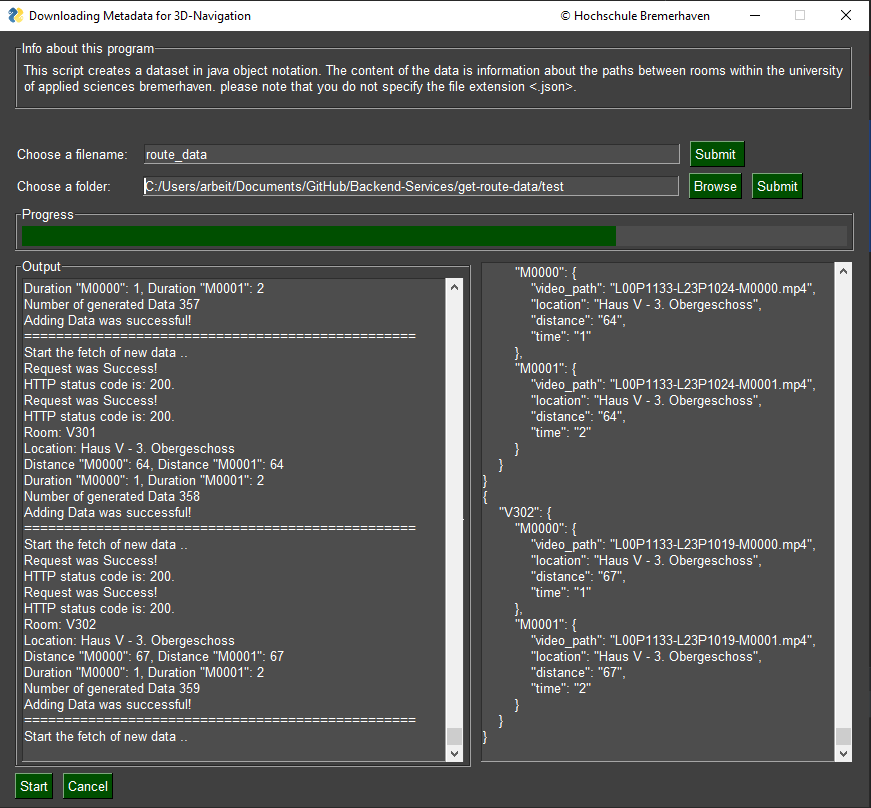
\includegraphics[width=\textwidth]{Figures/3DNavigator/create_metadata_pic_Fertig.png}
    \caption{Screenshot: Grafische Oberfläche des Metadata-Skripts}
    \label{fig:integration}
    \centering
\end{figure}\vspace{-2.5mm}

 % Skripte und Erweiterungen

\newcommand{\bigdatachapter}{Kapitel 9. }
\chapter{Big Data}
\label{chapter:big-data}
\lhead{\bigdatachapter \emph{Big Data}}

\section{Allgemein}
Wir haben in unserem Projekt ein großes Augenmerk auf das Sammeln von Daten gelegt. Big Data ist ein Thema, auf welches man in Zeiten wie diesen, in immer mehr Bereichen des Lebens stößt. Sei es die Kontaknachverfolgung, die Digitalisierung sämtlicher gesundheitlicher und behördlicher Dokumente, oder das Sammeln von Kundendaten.

Wir und unser Projekt zählt sich eher zum Letzteren und da wir nun schon auf die Quelle der Daten, Pepper und seine Kommunikation mit den Studenten und Interessierten, sowie auf die Verarbeitung und Speicherung mit Hilfe unserer Webanwendung eingegangen sind, wollen wir nun auch noch einmal aufzeigen, was man mit diesen Informationen anfangen kann. Einen kleinen Ausschnitt haben wir schon in den Abbildungen \ref{fig:admindashboard1}, \ref{fig:admindashboard2} und \ref{fig:webappdetail} gesehen. Doch dort ist nicht mehr, als die bloße Einsicht möglich.\\

\section{Datenanalyse mit Python und Jupyter Notebook}
Hier kam es uns zu Gute, dass wir uns mit Jupyter Notebooks sehr gut auskennen. Wir haben eine Client Klasse in Python geschrieben, welche es uns ermöglicht, durch bloße Eingabe des API Keys, auf Daten in unserer Webanwendung zuzugreifen. Hierfür wird der Endpunkt \verb|/docker-hbv-kms-http/api/v1/sql| angesprochen, an welchen wir unsere SQL Abfragen schicken können und die Ergebnisse als Antwort von unserer Webanwendung zurück bekommen.

Die Client Klasse sorgt automatisch dafür, dass die Anfragen entsrechend formatiert und abgeschickt werden, sowie Fehler ohne Probleme behandelt und mitgeteilt werden. Somit bekommt der Nutzer in seinem Jupyter Notebook mitgeteilt, sofern er einen Fehler in seiner SQL Syntax hat, da wir auch diese Informationen von unserem Server an den Benutzer übermitteln. Nachfolgend ist ein solches Beispiel vorgeführt:
\newpage

\begin{lstlisting}[language=Python, caption={Instantiierung des Clients und Ausführen einer SQL - Abfrage }]
    [ IN ]  client = Client(API_KEY, sandbox=False)
    [ OUT ] { 'message': 'Connected!' }
    [ IN ]  client.sql_query('select * from users')
    [ OUT ] Exception: 400-Invalid SQL command!
\end{lstlisting}

Wer sich an Abschnitt \ref{sec:api-sql-query} erinnert wird bemerken, dass die Tabelle \verb|users| nicht über diesen Endpunkt ansprechbar ist.

Der Parameter \verb|sandbox|, welcher im Konstruktor der Client Klasse verarbeitet wird, gibt an, ob sich mit der lokalen Instanz der Webanwendung, oder mit der in der Produktivumgebung verbinden werden soll.

Hat man nun die Client Klasse instantiiert, ist es mit ihr möglich eine Vielzahl von SQL Abfragen durchzuführen, um an verschiedene von Pepper gespeicherte Konversationsdaten zu gelangen.

Mit Hilfe der Bibliotheken Pandas, Matplotlib und weiteren Frameworks, haben wir innerhalb dieses Notebooks verschiedene Visualisierungen angefertigt. Hierbei ist zu beachten, dass all diese Daten mit Hilfe des Skriptes aus Abschnitt \ref{sec:dummy-data} generiert worden sind.\\

\begin{figure}[H]
    \centering
    \begin{minipage}[b]{0.49\textwidth}
        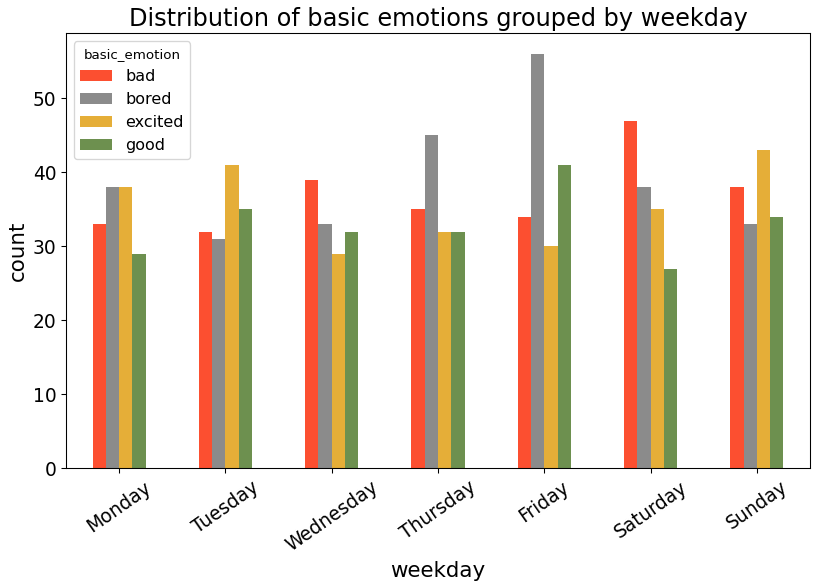
\includegraphics[width=\textwidth]{Figures/analysis/emotionwd.png}
        \caption{Diagramm: Emotion je Wochentag}
        \label{fig:emotionwd}
    \end{minipage}
    \hfill
    \begin{minipage}[b]{0.49\textwidth}
        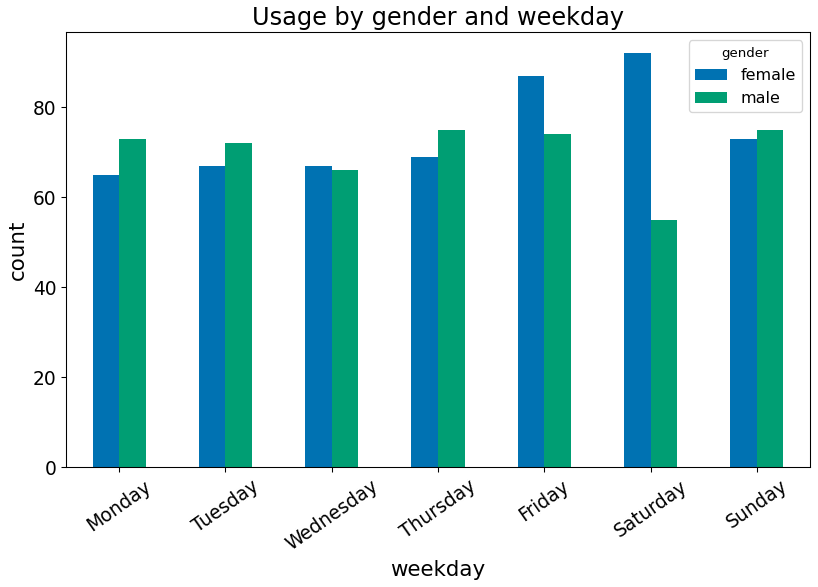
\includegraphics[width=\textwidth]{Figures/analysis/genderwd.png}
        \caption{Diagramm: Geschlecht je Wochentag}
        \label{fig:genderwd}
    \end{minipage}
\end{figure}

\begin{figure}[H]
    \centering
    \begin{minipage}[b]{0.49\textwidth}
        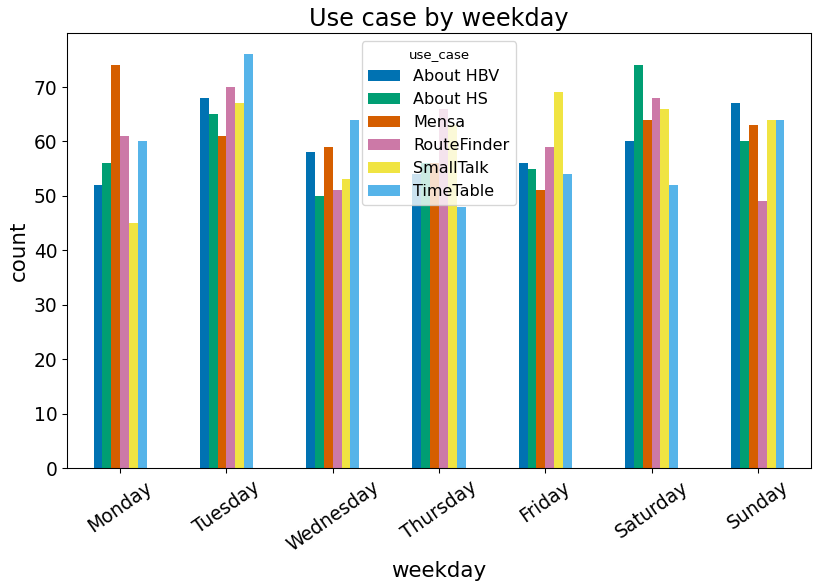
\includegraphics[width=\textwidth]{Figures/analysis/usecasewd.png}
        \caption{Diagramm: UseCase je Wochentag}
        \label{fig:usecasewd}
    \end{minipage}
    \hfill
    \begin{minipage}[b]{0.49\textwidth}
        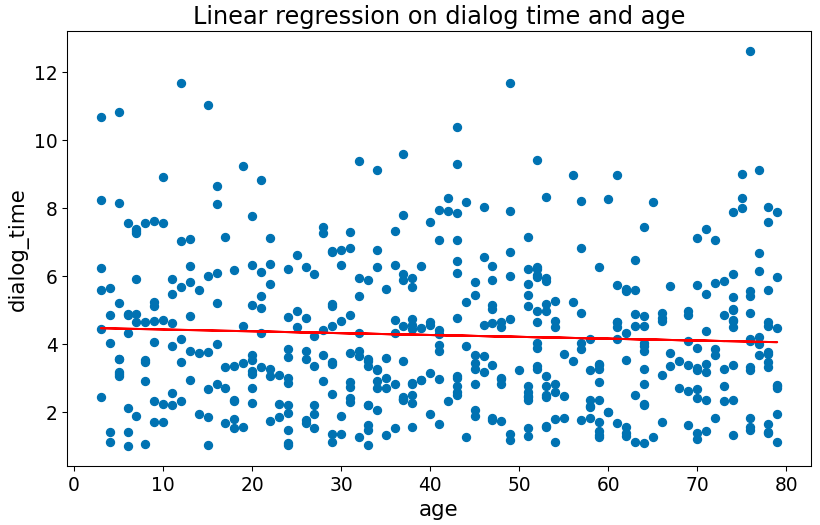
\includegraphics[width=\textwidth]{Figures/analysis/linreg.png}
        \caption{Diagramm: Lineare Regression zwischen Dialogzeit und Alter}
        \label{fig:linreg}
    \end{minipage}
\end{figure}

Die Abbildungen \ref{fig:emotionwd}ff. geben einen kleinen Vorgeschmack auf die Möglichkeiten der Analyse der von Pepper sammelbaren Daten. In dem Notebook sind weitere Diagramme zu finden, auch ein simples RNN wurde konstruiert, mit welchem wir das Alter anhand der zur Verfügung stehenden Parameter bestimmen wollten. Jedoch es nicht verwunderlich, dass wir bei einer Genauigkeit von 50\% liegen, da diese Daten von uns generiert worden sind.

Diese Schnittstelle zu unserem Webserver ermölgicht es dem Anwender, einen genaueren Einblick in die Daten zu bekommen. Zusätzlich zu diesem Notebook, haben wir ein Skript erstellt, welches die Daten aus der Datenbank abruft und die Visualisierungen als PDF Datei speichert. Dies ist in Verbindung mit einem Cronjob, einem wiederkehrenden Prozess, sehr nützlich. So können wir, aber auch andere, die diese Art der Anwendung nutzen wollen, sich in regelmäßigen Abständen, Berichte generieren lassen, welche einen tieferen Einblick in die Daten bieten.

Durch die Anbindung von Pepper an unsere Webanwendung ist es möglich, sämtliche Informationen, während einer Konversation zu speichern und nachzuvollziehen. Hiermit können Unternehmen herausfinden, was ihre Kunden bewegt und in welchen Bereichen man noch an seinem Geschäftsmodell arbeiten muss. Es wäre denkbar, mehrere Pepper, welche den selben Datensammlungsablauf haben, an verschiedene Unternehmen zu vermieten, womit man als Vermittler ein großes Kontingent an Informationen zu verschiedenen Branchen sammeln und auswerten kann.\\

 %  Big Data

\newcommand{\ausblickchapter}{Kapitel 9. }
\chapter{Ausblick}
\label{chapter:ausblick}
\lhead{\ausblickchapter \emph{Ausblick}}


%\section{Mögliche Erweiterungen}

%Es gibt einige Erweiterungsmöglichkeiten unserer Anwendung, welche wir im Rahmen dieses Projektes aus zeitlichen Gründen nicht umsetzen könnten, welche wir dennoch untersucht haben und deswegen nicht unerwähnt lassen möchten.
Wir haben im Rahmen unseres Bachelorprojektes gemerkt, dass Pepper in Kombination mit verschiedenen Frameworks und Tools zur Sammlung und Speicherung von Daten, ein enormes Erweiterungspotenzial bietet. Um auch auf die Möglichkeiten zum Ausbau unserer Arbeit aufzuzeigen, werden wir nun im Folgenden die für uns interessantesten Punkte darlegen.\\
\section{Google Dialogflow}

Dialog Flow ist eine von dem Konzern Google betriebene Plattform, welche das Verarbeiten und verstehen von menschlicher Sprache ermöglicht. Sie bietet den Vorteil, dass die Verarbeitung der Sprache nicht mehr auf dem eigenen System stattfinden, sondern an einen von Google bereitgestellten Server gesendet wird. Dieser verarbeitet die Daten und sendet sie anschließend wieder zurück. Dialog Flow hat dabei den Vorteil, dass sich die Interaktion der Dialoge dynamisch auf der von Google erstellten Browser-Plattform bearbeiten lassen. Eine Implementierung in das Pepper System könnte so das produktive Arbeiten stark verbessern. Es ist außerdem möglich, Lernraten zu definieren, durch welche Pepper ohne das erneute Aufspielen einer Applikation dazu lernen könnte. Pepper wäre mit einer solchen Architektur in der Lage, selbst und dynamisch dazuzulernen und seine Interaktion und das Verstehen von Wörtern und Sprache ständig weiter zu optimieren. Wir haben für diese Funktionalität ein grafisches Konzept erstellt, welches den Ablauf dieser theoretischen Funktionalität verdeutlichen soll:

\begin{figure}[H]
    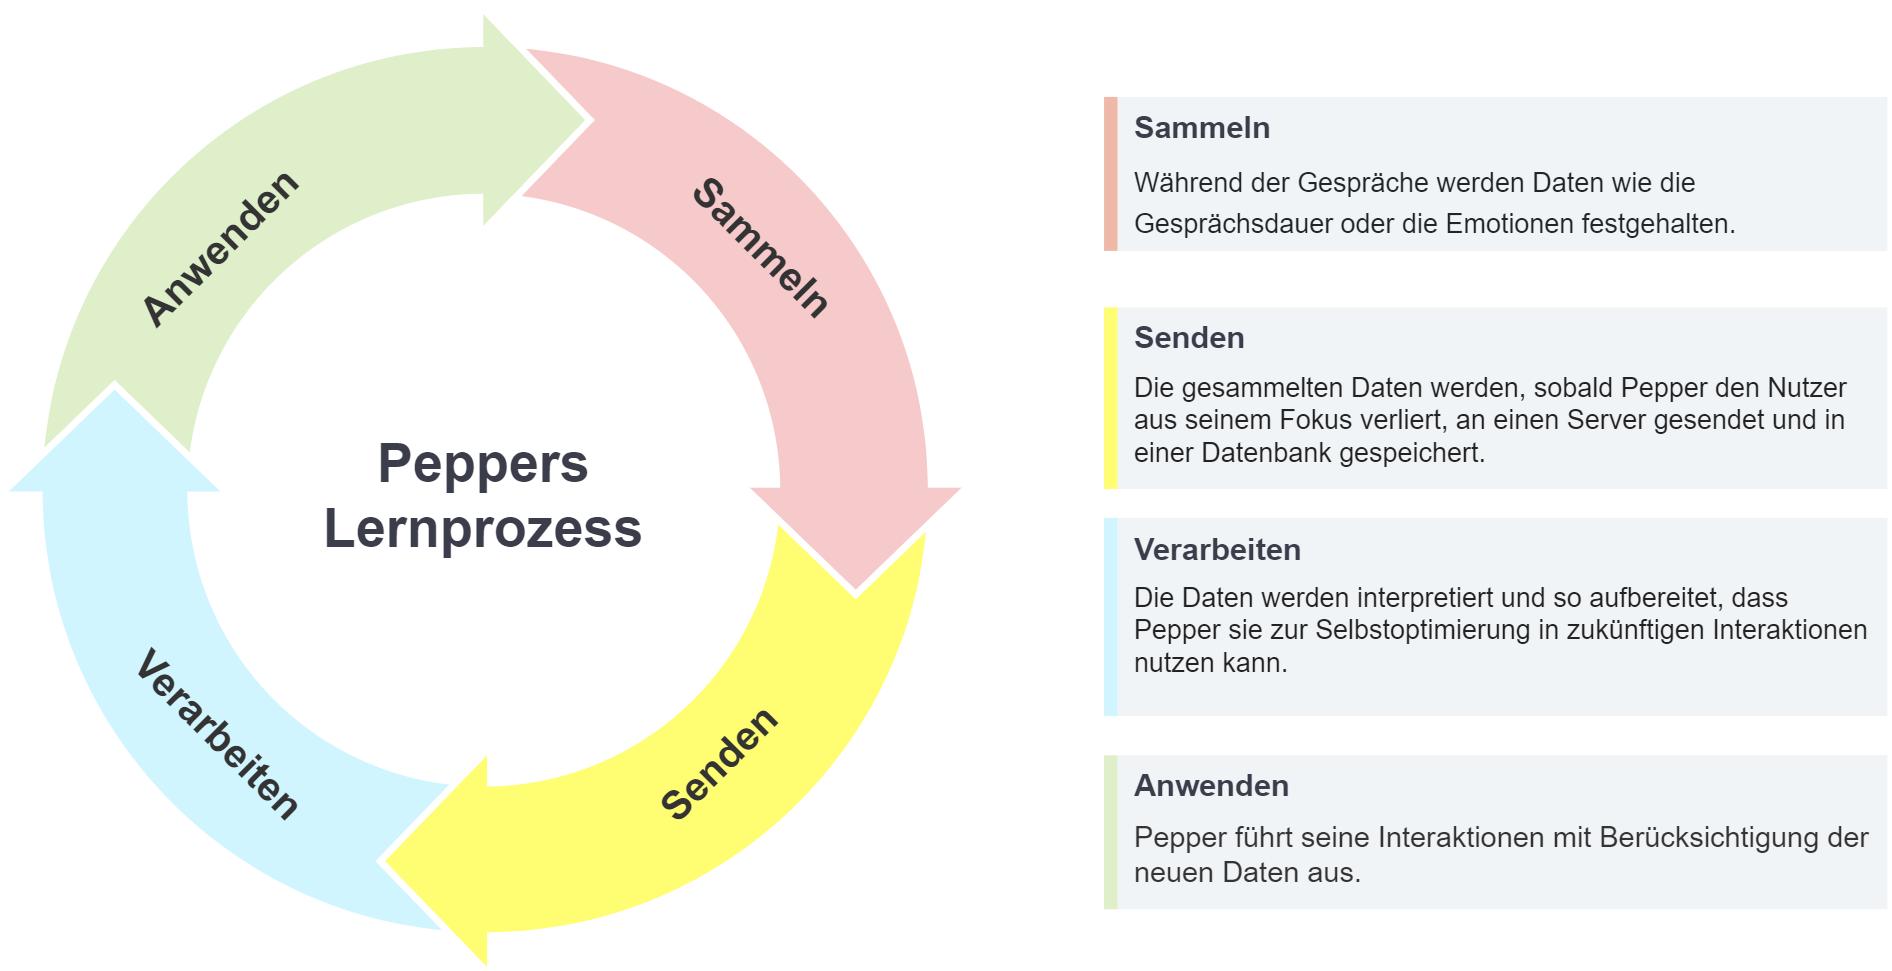
\includegraphics[width=\textwidth]{Figures/pepper-lerprozess.png}
    \caption{Diagramm: Lernprozess}
    \label{fig:integration}
    \centering
\end{figure}

Obwohl es eine von SoftBanks-Robotik offiziell bereitgestellte Schnittstelle für eine Anbindung an die Google-Dialogflow Plattform gibt, haben wir uns nicht nur aus zeitlichen Gründen gegen die Entwicklung einer solchen Funktionalität entschieden. Dabei gab es für uns zwei entscheidende Faktoren. Erstens empfinden wir es als äußerst unpassend, unser bereits entwickeltes System, welches dem Administrator den Vorteil bietet, die gesammelten Daten selbst zu besitzen, mit einer Anwendung zu verknüpfen, durch welche diese an einen Großkonzern weitergegeben werden. Das würde für uns bedeuten, dass wir einen unserer bedeutendsten Schwerpunkte dieser Arbeit verlieren, und zwar das ermöglichen gesammelte Daten selber zu verwalten und beliebig in eigene Dateiformate zu konvertieren und weiterzuverarbeiten. Außerdem ist es so, dass Google die Dialogflow Plattform nur für zahlende Kunden in Form eines Abo-Modells anbietet, wobei hier Mikrobeträge pro Request an die Plattform bezahlt werden müssen. Es wäre also alleine schon ein Kostenfaktor, eine Anwendung, während des Entwicklungsprozesses mit diesem System zu testen. Trotzdem möchten wir der Vollständigkeitshalber auf die Möglichkeit der Anbindung an Google Dialog hinweisen, auch wenn sie sich nicht mit den Ethischen-Vorstellungen unserer Softwareanwendung vereinbaren lassen.\\

\section{Dynamisches Bewegen im Raum}

Es ist möglich, Pepper das Bewegen in einem Raum beizubringen. Dies würde den Roboter für den Benutzer noch menschlicher erscheinen lassen, da es den Roboter um die Eigenschaft der Proxemik erweitern würde. Außerdem könnte Pepper so Routen ablaufen, um evtl. noch mehr Benutzer für die Interaktion zu finden und diese auf sich aufmerksam zu machen. Auch das automatische Ansteuern einer Ladestation wäre durch diese Funktion möglich, wodurch Pepper autonomer und noch unabhängiger von der Betreuung eines Menschen während seiner Arbeit wird.\\

\section{Socialmedia - Bot}
\label{sec:Sozialmedia-Bot}
Während der Arbeit an und mit Pepper fiel uns vor allem das außerordentliche Interesse auf, welches bei Passanten zu beobachten war. Es kam zudem des Öfteren vor, dass der Roboter gefilmt wurde oder man uns fragte, ob es möglich sei ein “Selfi” mit dem Roboter zu machen. Die von Pepper ausgelöste Neugier bei Menschen hat, inspirierte uns zu dem Konzept, den Roboter selbst als Social-Media-Marketing Instrument einzusetzen.
Ein solcher Anwendungsfall wäre durch die Implementierung eines oder mehrerer Bots (automatisierter Accounts) in die Architektur unserer Anwendung umsetzbar. Es wäre somit möglich, dass der Roboter bewusst Benutzer dazu auffordert, mit ihnen zu interagieren und ein Selbstporträt zu machen. Im Anschluss daran könnte der Bot mit einem zufällig gewählten Kommentar auf das veröffentlichte Bild regieren, wenn er erkennt, dass er auf diesem verlinkt wurde. Außerdem könnte der Bot selbstständig Veröffentlichungen aus den von ihm gesammelten Daten erstellen, in welchem er diese visuell darstellt und interpretiert. Pepper könnte so für seinen Besitzer einen positives Marketingeffekt erzielen.\\

\section{Weitere potenzielle Einsatzbereiche}

Wir haben während der Entwicklung mit Pepper, noch eine Reihe weitere Anwendungsfälle für unsere Software-Architektur definiert. Drei dieser Einsatzbereiche haben wir im Folgendem aufgelistet.\\

\subsection{Gastronomie}

Es könnte ein System wie das aus dem Bachelor-Projekt mit Pepper als Möglichkeit zum Daten sammeln für die Gastronomie interessant sein. Pepper könnte Kunden zu ihrer Zufriedenheit befragen, Bestellungen aufnehmen oder über das Hygienekonzept informieren. Die dabei gesammelten Daten lassen sich flexibel analysieren, um ein genaueres Bild über die Kunden zu ermitteln und dies für potenzielle Optimierung von Geschäftsprozessen zu einzusetzen.\\

\subsection{Krankenhäuser und Pflegeeinrichtungen}

Pepper, könnte viele zwischenmenschliche Aufgaben in einem Pflegeheim erfüllen. Zudem wäre es mit der von uns entwickelten Software-Architektur möglich, den gesundheitlichen Zustand und das generelle Wohlbefinden eines Bewohners einzuordnen und anschließend zu auf einem Server zu dokumentieren. Der Roboter könnte die Menschen in einer Einrichtung dabei spielerisch im Alltag unterstützen, während er Daten über die physische, sowie psychische Befindlichkeit sammelt. Wie die Daten können anschließend von Mitarbeitern des Pflegeheims ausgewertet werden.\\

\subsection{Kaufhäuser}

Große Einkaufszentren könnten die Anwendung ähnlich nutzen, wie wir es in unserem Entwurf für die Hochschule getan haben. Der Roboter würde Wegrouten beschreiben oder über das Kaufhaus informieren. Zusätzlich wäre es hier auch von Nutzen, den Roboter um ein Konzept wie in \ref{sec:Sozialmedia-Bot} beschrieben zu erweitern. Außerdem könnte Pepper so programmiert werden, dass er Anfragen zu spezifischen Produkten entgegennimmt, um dem Benutzer die entsprechenden Geschäfte zu nennen, in welchen es dieses zu erwerben gibt.\\

 % Ausblick

\chapter{Abschließende Worte}
\label{sec:zusammenfassung}
\lhead{Kapitel 10. \emph{Abschließende Worte}}

Die Arbeit mit Pepper hat uns die Relevanz und den großen Nutzen eines humanoiden Roboters 
verdeutlicht. Außerdem hat sich für uns gezeigt, dass vor allem die Interaktion zwischen dem 
Benutzer und der Software durch einen humanoiden Roboter stark verbessert wird. 

Wir haben im Laufe des Projektes sehr viele und zum Teil neue Erfahrungen mit verschiedenen Softwares und Tools sammeln können. Die Entwicklung einer Anwendung für einen auf Andriod basierenden Roboter, sowie die vollständige Entwicklung von zwei Webservern mit unterschiedlichen Backends, haben uns aufgezeigt, welches Potential uns durch die freie Gestaltung unseres Bachelorprojektes geboten wurde. Dies gilt auch für die kleinen Skripte, die wir zur Ermittlung der Mensa- oder Routeninformationen entwickelt haben.

Auch die Arbeit im Team war sehr angenehm. Wir haben zum Teil täglich miteinander
den Diskurs gesucht, neue Ideen ausgetauscht miteinander gearbeitet. Hierbei konnte
jeder etwas von dem Anderen lernen, sodass nach einem Treffen alle etwas schlauer
und mit einem guten Gefühl den Jitsi Raum verlassen konnten.

Das Potential von Pepper ist größer als wir zu Anfang dachten, da dieser für die verschiedensten Anwendungsfälle 
programmiert werden kann. Bei der Planung der einzelnen Anwendungsfälle für die Hoschule Bremerhaven ist uns
dies schon aufgefallen, da wir viele weitere Ideen bekommen haben, was noch implementiert werden könne. Viele
Dieser Ideen würden wären jedoch über den Rahmen eines Bachelorprojektes hinaus gegangen. Hätten wir die Entwicklungsumgebung
ROS verwenden können, wäre das Potential noch größer, da man auch auf die einzelnen Kameras und Sensonren zuzugreifen. % Abschließende Worte





%% ----------------------------------------------------------------
% Now begin the Appendices, including them as separate files

%\addtocontents{toc}{\vspace{2em}} % Add a gap in the Contents, for aesthetics

%\appendix % Cue to tell LaTeX that the following 'chapters' are Appendices

%\input{./Chapters/AppendixA}	% Appendix Title

%\input{./Chapters/AppendixB} % Appendix Title

%\input{./Chapters/AppendixC} % Appendix Title

%\addtocontents{toc}{\vspace{2em}}  % Add a gap in the Contents, for aesthetics
%\backmatter

%% ----------------------------------------------------------------
\label{Literaturverzeichnis}
\lhead{\emph{Literaturverzeichnis}}  % Change the left side page header to "References"

\bibliographystyle{plainnat}  % Use "unsrtnat" BibTeX style for formatting the references

\bibliography{references}  % The references information are stored in the file named "references.bib"

\nocite{*}

\end{document}
%% ----------------------------------------------------------------
